\documentclass[a4paper,twoside,11pt]{article}
\usepackage{a4wide,graphicx,fancyhdr,clrscode,tabularx,amsmath,amssymb,color,enumitem}
\usepackage{algo}
\usepackage{bm}
\usepackage{indentfirst}
\usepackage{hanging}
\usepackage[round]{natbib}
\usepackage{amsmath,amssymb}
\usepackage{lscape}
\usepackage{booktabs}
\usepackage{setspace}
\usepackage{makecell}
\usepackage{dcolumn}
\usepackage{longtable}
\usepackage{caption}
\usepackage{tocbasic}
\usepackage{tablefootnote}
\usepackage{array}
\usepackage{hyperref}
\usepackage{subcaption}
\usepackage{graphbox}
\usepackage{tabularx}
\usepackage{threeparttable}
\usepackage[labelfont=sc]{caption}
\usepackage[section]{placeins}
\newcolumntype{P}[1]{>{\centering\arraybackslash}p{#1}}
\newcolumntype{M}[1]{>{\centering\arraybackslash}m{#1}}
\renewcommand*{\listoffigures}{\listoftoc[\listfigurename]{lof}}
\renewcommand*{\listoftables}{\listoftoc[\listtablename]{lot}}
\setuptoc{lof}{leveldown,totoc}
\setuptoc{lot}{leveldown,totoc}
\makeatletter
\newcommand*{\rom}[1]{\expandafter\@slowromancap\romannumeral #1@}
\makeatother
\raggedbottom
\FloatBarrier
%----------------------- Macros and Definitions --------------------------
\renewcommand{\baselinestretch}{1.25}
\setlength\headheight{20pt}
\addtolength\parindent{1em}
\addtolength\topmargin{-10pt}
\addtolength\footskip{20pt}

\fancypagestyle{plain}{%
\fancyhf{}
\fancyhead[LO,RE]{\sffamily UC DAVIS ARE}
\fancyhead[RO,LE]{\sffamily Progress Report}
\fancyfoot[LO,RE]{\sffamily}
\fancyfoot[LO,RE]{\sffamily \thepage}
\renewcommand{\headrulewidth}{0pt}
\renewcommand{\footrulewidth}{0pt}
}

\pagestyle{fancy}
\fancyhf{}
\fancyhead[LO,RE]{\sffamily}
\fancyhead[RO,LE]{\sffamily}
\fancyfoot[LO,RE]{\sffamily}
\fancyfoot[LO,RE]{\sffamily \thepage}
\renewcommand{\headrulewidth}{0pt}
\renewcommand{\footrulewidth}{0pt}

\newcommand{\R}{{\mathbb R}}
\newcommand{\N}{{\mathbb N}}
\newcommand{\Z}{{\mathbb Z}}
\newcommand{\Q}{{\mathbb Q}}
\allowdisplaybreaks


\begin{document}
\title{\vspace{0.8\baselineskip} 
\textsc{Research in Progress} \\ The Impact of Electronic Benefit Transfer on WIC Participation: Evidence from Natality Data}
\author{Charlotte Ambrozek \\ UMN \and Timothy K.M. Beatty \\ UC Davis \and Wenjie Zhan \\ UC Davis}
\maketitle

\begin{abstract}
Between 2002 and 2022, the Special Supplemental Nutrition Program for Women, Infants, and Children
(WIC) transitioned from paper vouchers to electronic benefit transfer (EBT) cards. This payment reform
was expected to encourage WIC participation by reducing transaction costs and welfare stigma but empirical evidence has been mixed. One challenge in prior work is absence of detailed WIC participation data on a large scale, limiting
the generalizability of results. In this paper, we evaluate the impact of WIC EBT implementation on WIC
participation by linking the WIC EBT roll-out schedule across virtually all counties in the U.S. to natality
data, which began reporting WIC participation in 2009. We document a significant increase in WIC participation among births that are most likely eligible for WIC: after the implementation of EBT, WIC participation among the births of less educated and unmarried mothers increases by 9.18\%, and by 14.82\% if the mothers are also black or Hispanic. Our results are robust to sample selection, estimation methods, and definitions of likely eligible sub-population. We also reconcile our results with seemingly opposite results in \cite{meckel2020cure}.
\end{abstract}

\clearpage
\section{Introduction}
The Special Supplemental Nutrition Program for Women, Infants, and Children
(WIC) provides nutritious foods and nutrition counseling for low-income pregnant or postpartum women, infants, and children under the age of five. To be eligible for WIC, one needs to live in households with family incomes under 185\% of federal poverty line or have participated in other welfare programs such as Medicaid, Temporary Assistance to Needy Families (TANF), or Special Supplemental Nutrition Program (SNAP).  WIC participation has been linked to improved birth and children outcomes \citep{hoynes2011can,kreider2016identifying,chorniy2020does}. However, total WIC participation has been declining by approximately 3 millions in last decade. In 2009, WIC served around half of all infants born in the U.S. This number dropped to 30\% in 2021 (as in Figure \ref{trend1}). Between 2002 and 2022, WIC transitioned from paper vouchers to electronic benefit transfer (EBT) cards. This payment reform was expected to encourage WIC participation by reducing transaction costs and welfare stigma associated with using paper vouchers. Empirical evidence, on the other hand, shows mixed findings. For example, \cite{hanks2019paper} find that WIC EBT increases WIC
redemption in Ohio. \cite{li2022impacts} find no significant impact of WIC EBT on the share of WIC enrollment in Oklahoma. Finally, \cite{meckel2020cure} finds WIC EBT decreases the number of WIC births in Texas. One common concern in previous work is that results are based on individual states thus difficult to generalize. In this paper, we evaluate the impact of WIC EBT implementation on WIC participation by linking the WIC EBT roll-out schedule across virtually all counties in the U.S. to Vital Statistics Natality Data, which began reporting WIC status of live births in 2009. Live births participated in WIC (henceforth, WIC births) can plausibly capture the change in total WIC participation because the ratio of WIC births to total WIC participants maintain 20\% from 2009 (as in Figure \ref{trend2}). The share decline mildly after pandemic, but we show that our results do not change after dropping data after 2019.

\begin{figure}
	\begin{subfigure}[t]{.5\textwidth}
		\centering
		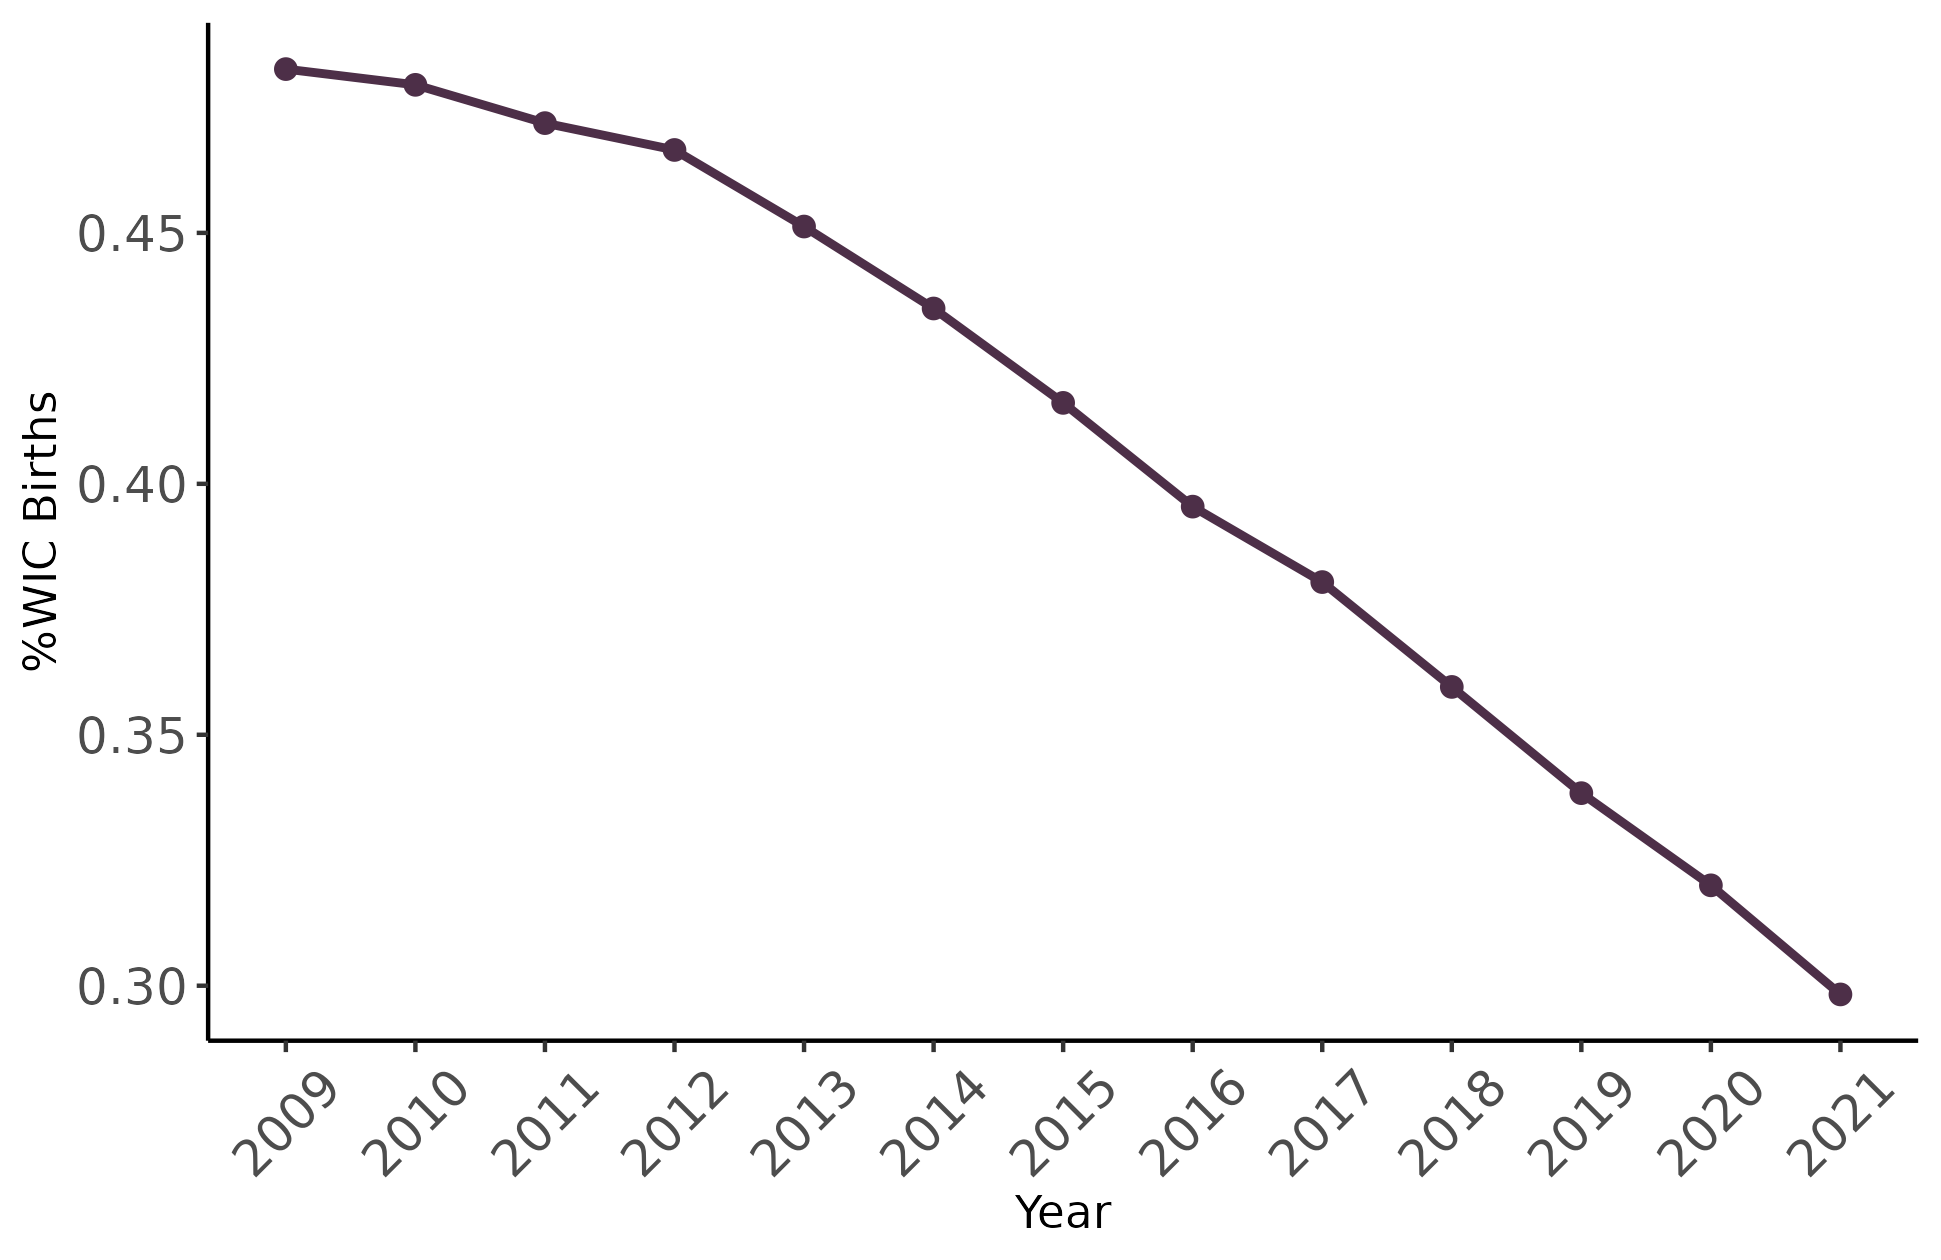
\includegraphics[width=\textwidth]{wic_par_sum_res.png}  
		\caption{\% Births Participated in WIC}
		\label{trend1}
	\end{subfigure}
	\begin{subfigure}[t]{.5\textwidth}
		\centering
		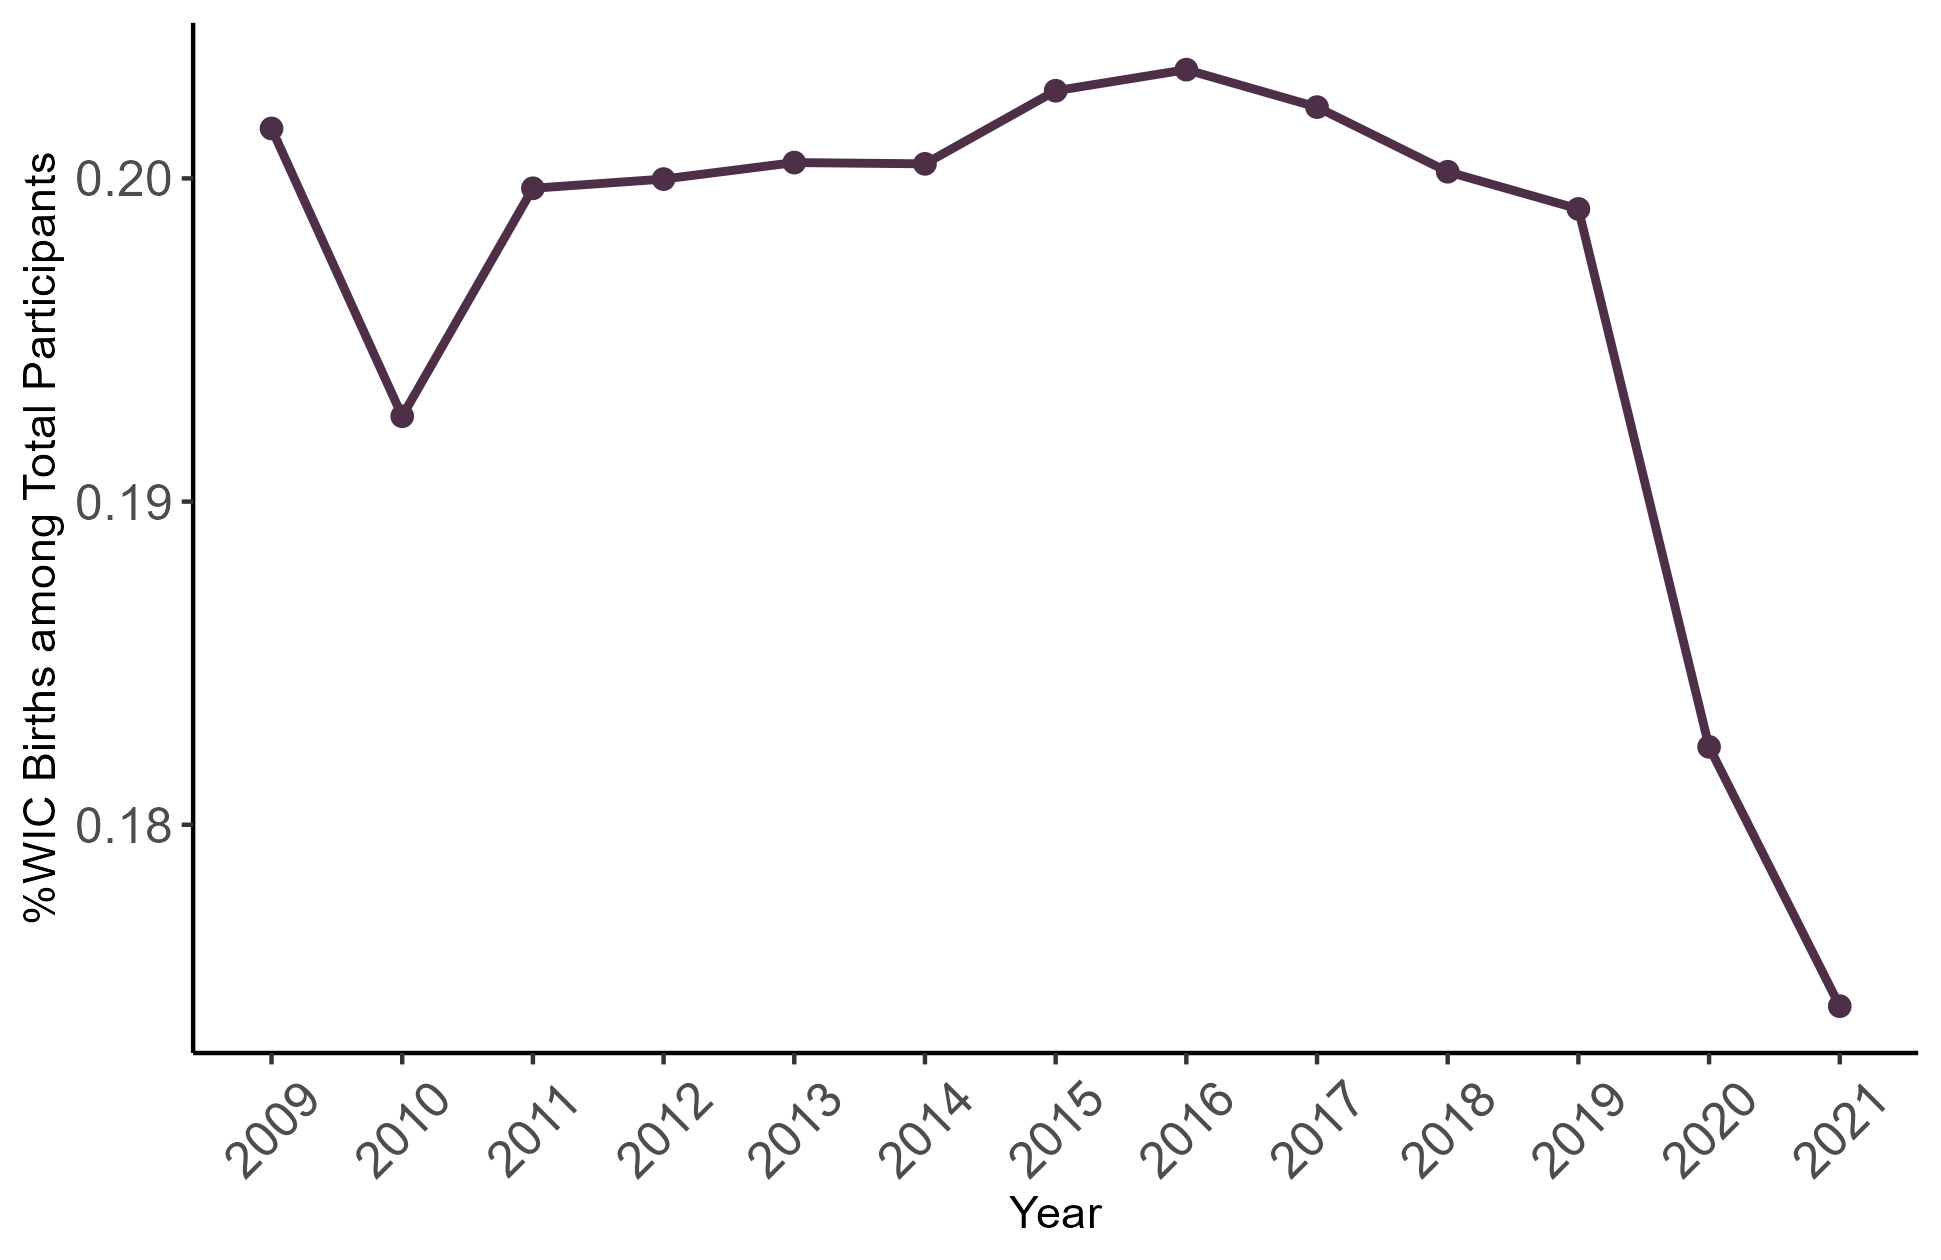
\includegraphics[width=\textwidth]{wic_par_pc.png}  
		\caption{The Ratio of WIC Births to All Participants}
		\label{trend2}
	\end{subfigure}
	\caption{\textsc{Trends of WIC Births}}
	\label{trend}
	\footnotesize
\end{figure} 

This paper builds on \cite{meckel2020cure}, which leverages WIC EBT rollout in Texas to study both vendors' and consumers' responses to EBT transition. She finds that EBT implementation causes vendors to drop out and reduces program take-up. We extend Meckle's analysis on program take-up to national level by collecting WIC EBT roll-out schedule across virtually all counties in the U.S. Our preferred estimates show results opposite to Meckle's findings in Texas: WIC EBT significantly increase WIC participation among mothers who are more likely eligible for WIC. Specifically, WIC participation increase by 9.18\% among less-educated and unmarried mothers after EBT implementation and by 14.82\% if the mothers are also minority. We find that Meckle's results on WIC take-up pick up the trend of numbers of live births and thus cannot tease out causal impact of EBT. Our preferred estimators using Meckle's data show that impact of EBT on WIC participation in Texas is in fact consistent with our main results based on much larger amounts of counties. Our results are robust to sample selection, estimation methods, timing of data collection, and definition of likely eligible sub-population.

We make several contributions to existing literature. First, we contribute to literature evaluating impacts of WIC EBT by collecting nationwide, county-level EBT rollout schedule and providing more credible empirical evidence based on much larger sample. Second, we add to literature on behavioral response to detail change in the design of food assistance programs. Finally, we contribute to literature discussing factors affect take-up of public program.

\section{Data}
\subsection{Vital Statistics Natality Data}
Our data on WIC births is taken from restricted-use Vital Statistics Natality Database. Natality data is coded from birth certificates, which includes birth and parental information such as county of maternal residence, year of birth, and mothers' age, educational attainment, marital status, and WIC participation, etc. The 2003 revision of birth certificate requires addition of mothers' WIC participation. But this information was not available until 2009. We collapse the birth-level natality data to
county-of-maternal-residence-by-year-of-birth cells to make the sample size more manageable. Our sample period spans 2009-2021.

Ideally, we would like to construct our sample with only mothers eligible for WIC. Since we do not observe WIC eligibility or maternal income from birth certificate, we focus on less-educated and unmarried (LEUM) mothers as they are more likely to be eligible for WIC. This is a common approach to study policy impacts when we cannot tell who is the target of policy \citep{meckel2020cure,alsan2022fear, east2023labor}. \cite{meckel2020cure} create a "high poverty" indicator taking into account whether mother is non-white Hispanic or black, whether mother is unmarried, and whether mother has a high school education or less as a proxy for maternal income. We choose LEUM status over this high poverty indicator because a nontrivial amount of counties in our sample have few births to qualified mothers, especially the minority (as in Figure \ref{proxy}). To still be able to capture lower-income mothers while removing minority as one of the criteria, we focus on those with more restrictive educational backgrounds: mothers with less than high school education. Indeed, WIC participation rate among LEUM mothers is 73.62\%, similar to the participation rate among \cite{meckel2020cure}'s sample (79.90\%), and much higher than the total participation among all mothers, which is 43.15\%. We test sensitivity of our results to alternative proxies.

\begin{figure}
	\begin{center}
		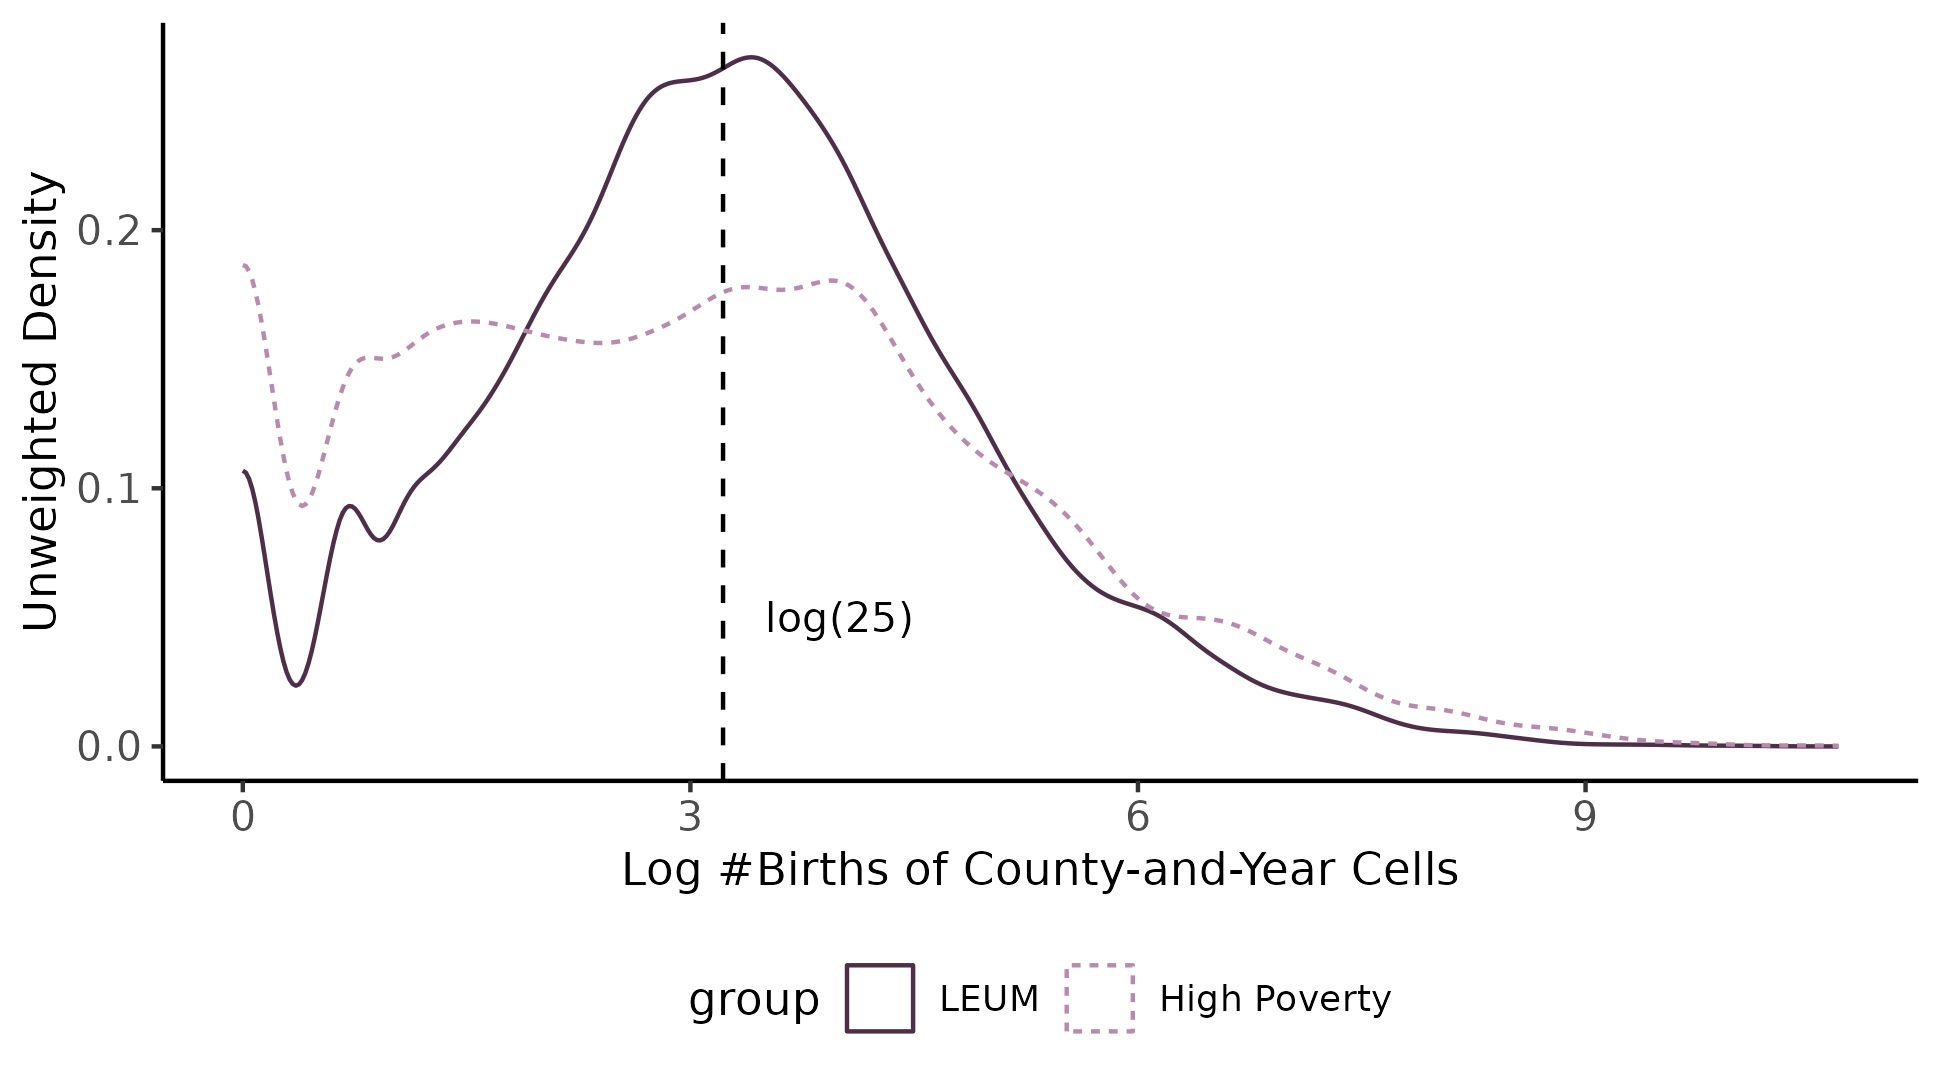
\includegraphics[width=.8\textwidth]{leum_hp.png}  
		\caption{\textsc{Comparing LEUM and High Poverty as Lower Limits for Cells}}
		\label{proxy}
	\end{center}
	\footnotesize
	Notes: The dashed line represents the distribution from the overlapped subset of \cite{meckel2020cure}'s data set. The solid line represents the distribution from the overlapped subset of our data set. They are almost identical.
\end{figure}

We validate our data by cross-checking whether the natality data from Vital Statistics are consistent with the birth data from Texas Department of State Health Services (Texas DSHS) used in \cite{meckel2020cure}. \cite{meckel2020cure}'s natality data from Texas DSHS covers births in counties implementing WIC EBT before April 2009 (239 counties) from January 2005 to December 2009. Our natality data covers births in all counties in Texas (254 counties) but only traces back to January 2009. Therefore, the overlapped subsets of two data sets cover births in counties implementing WIC EBT before April 2009, from January 2009 to December 2009. We compare the overlapped subsets of two data sets and find they are almost identical (as in Figure \ref{check}). 

\begin{figure}
	\begin{center}
		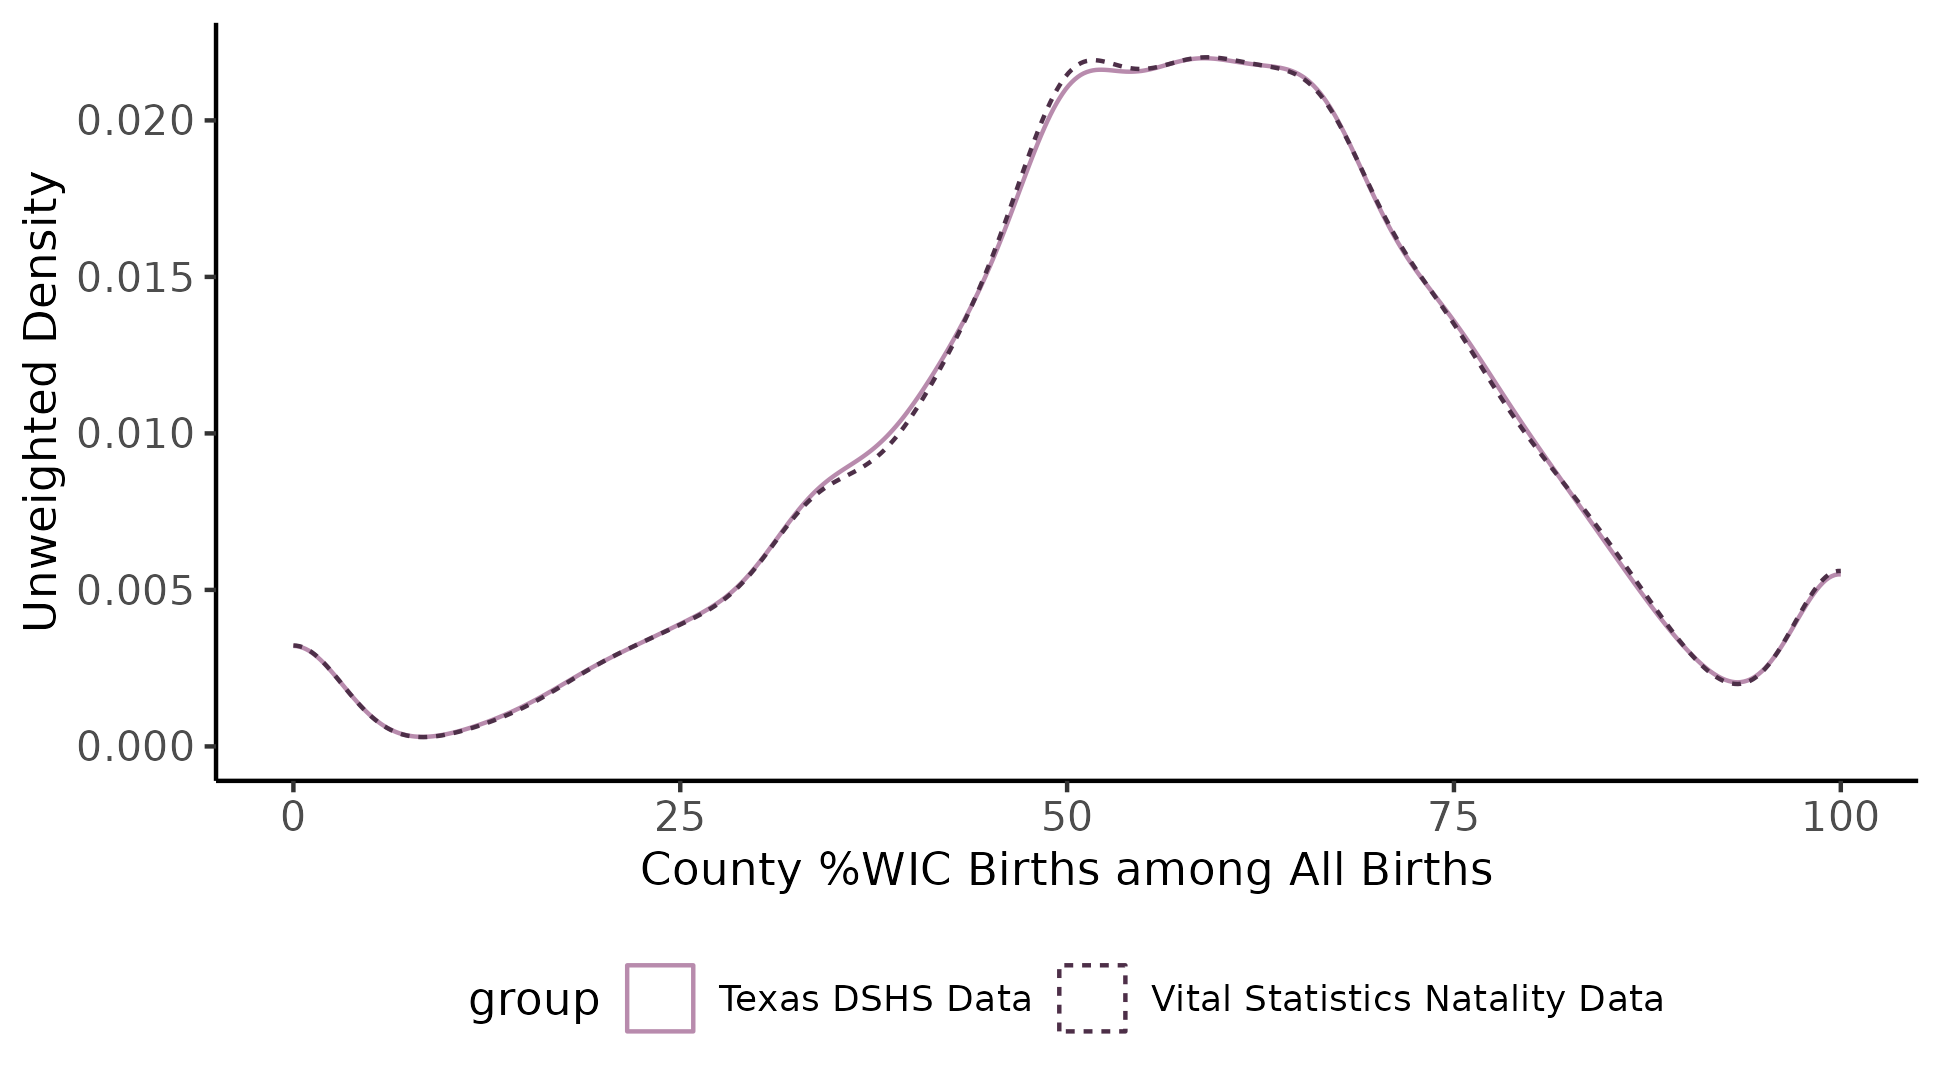
\includegraphics[width=.8\textwidth]{density_wic_rate.png}  
		\caption{\textsc{Distribution of County-level Share of WIC Birth}}
		\label{check}
	\end{center}
	\footnotesize
\end{figure}

\subsection{WIC EBT Roll-out}
We compile the WIC EBT rollout schedule across virtually all counties\footnote{Indian Tribal Organizations with separate WIC EBT implementation plans are excluded.} in the U.S. from public record of state WIC agencies. For counties reporting a range of implementation dates, we use the start date of that range. The county-level WIC EBT rollout is in Figure \ref{map}. We observation both cross- and within-state variation in timing of WIC implementation with cross-state variation dominating. Further excluding counties without reporting WIC participation, we end up a sample covering 2,549 counties, accounting for in total 81.24\% of population and 79.10 \% of births. Table \ref{included} presents baseline characteristics \footnote{These county baseline characteristics are chosen as they are likely to be correlated with the timing of WIC EBT implementation.} of our sample counties compared to those excluded counties. Included counties are not in general better off than excluded ones. Although included counties have smaller share of disadvantaged population, smaller share of infants with low birth weight, and receive more income maintenance benefits per person, they receive less SNAP benefit and have lower income per person. We do not observe significant difference in population size, per person reception of public assistance medical benefits, and net increase in WIC vendors between included and excluded counties. Table \ref{ebt_det} indicates that, while some county baseline characteristics are strongly correlated with the timing of WIC EBT implementation, they as a whole only explain a small share of the variation in implementation timing. Most of the variation in the timing of WIC EBT implementation is explained by state-level unobservables as R$^2$ becomes very close to 1 when state fixed effect is added. Therefore, the timing of the WIC EBT rollout can be considered plausibly exogenous after controlling for the county baseline characteristics.

\begin{figure}
	\begin{center}
		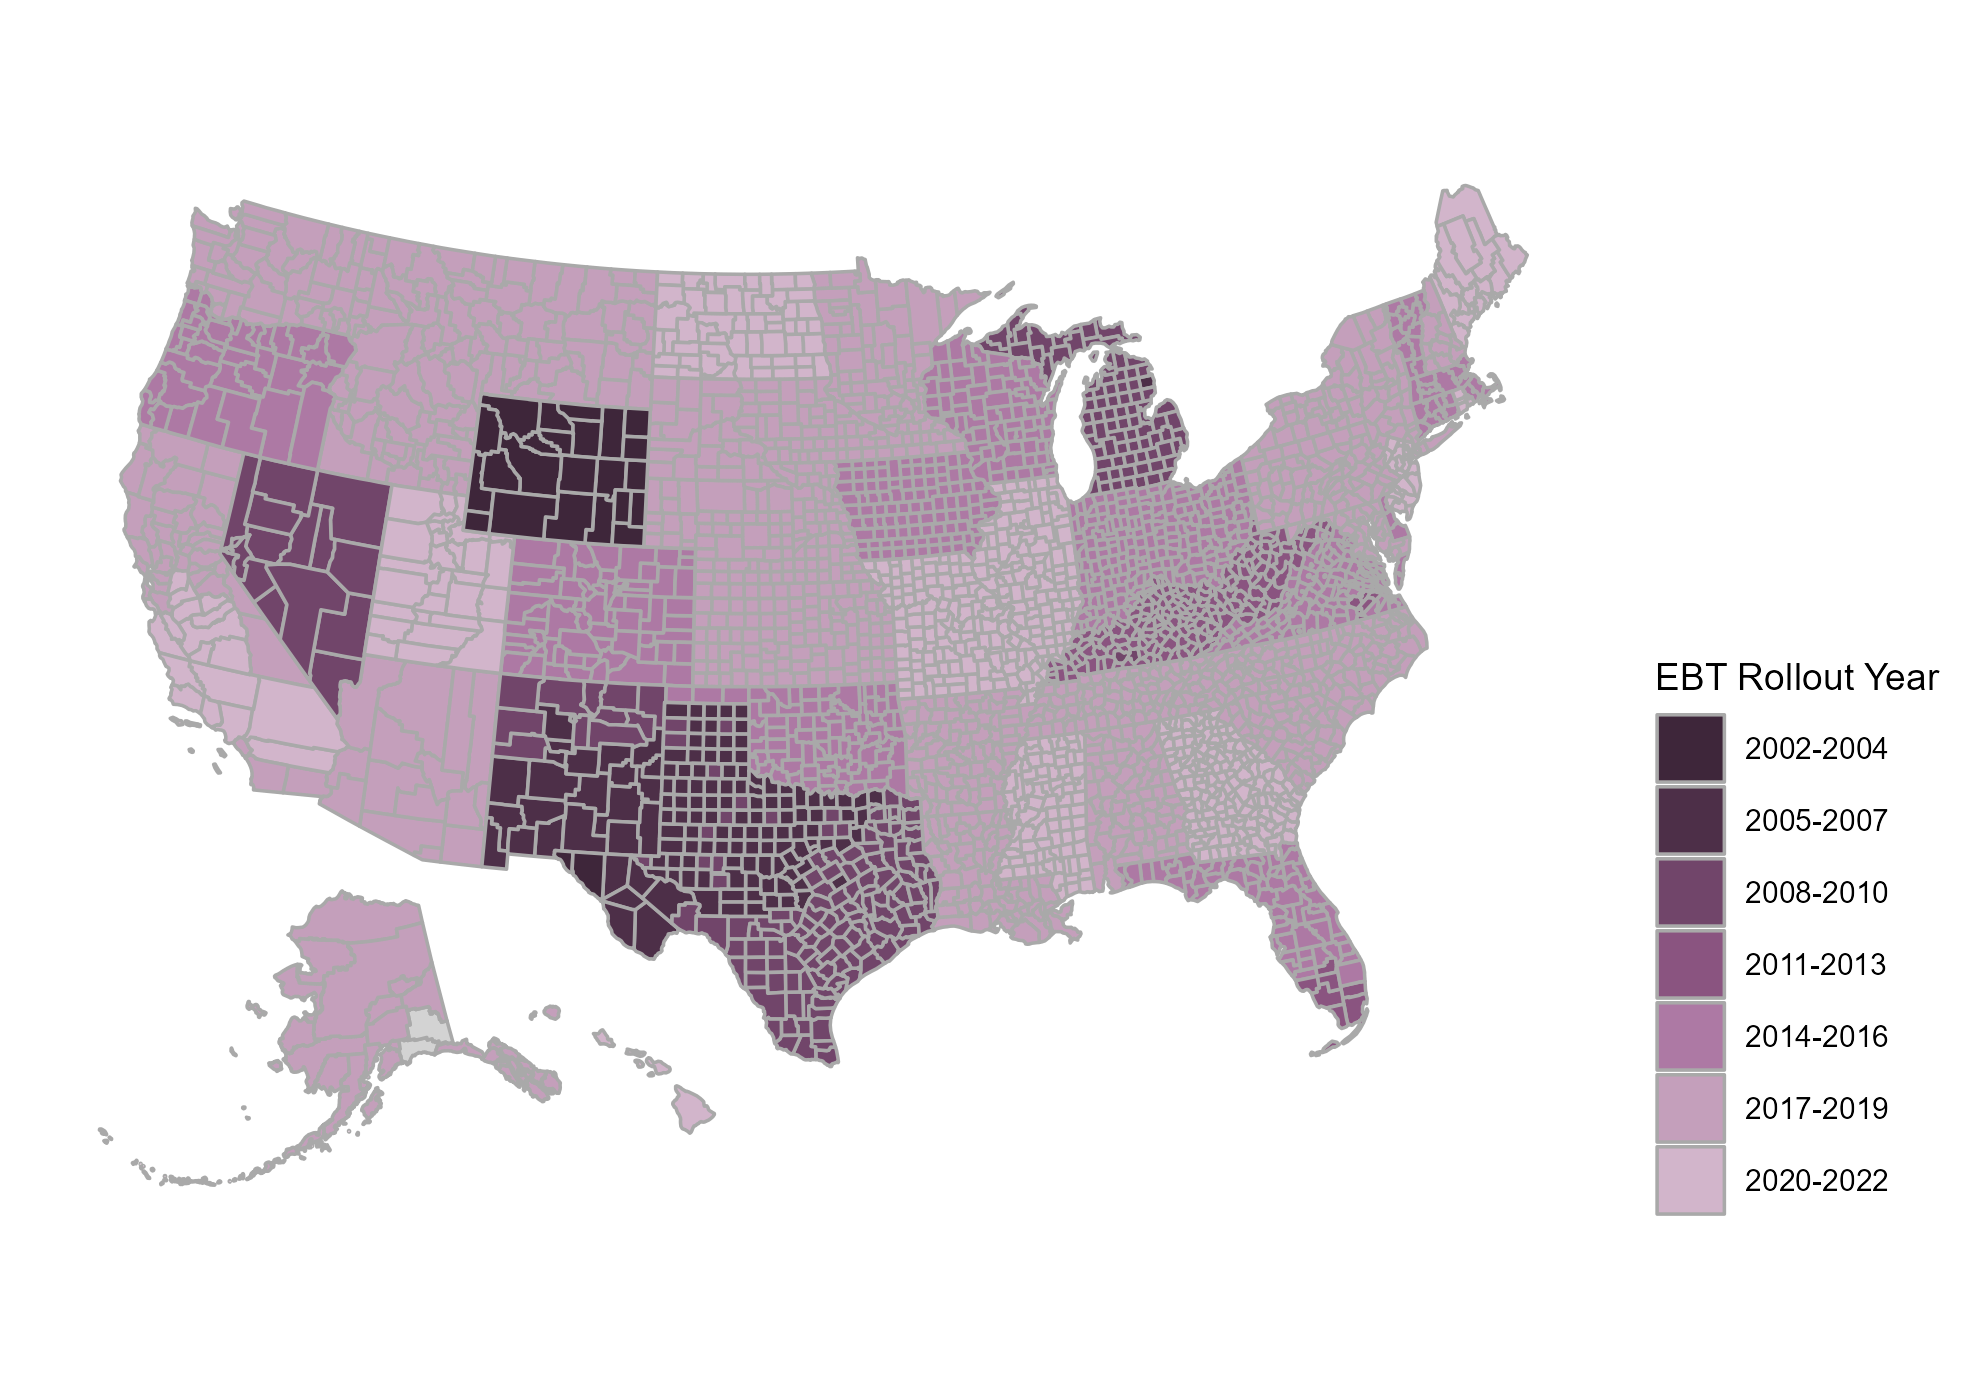
\includegraphics[width=.8\textwidth]{ewic_rollout_county_year.png}  
		\caption{\textsc{WIC EBT Roll-out Schedule}}
		\label{map}
	\end{center}
	\footnotesize
\end{figure}


\begin{table}[!htbp] 
	\begin{center}
		\caption{\textsc{Baseline Characteristics of Counties Included and Excluded in Sample}} 
		\label{included} 
		\footnotesize 
		\begin{tabular}{@{\extracolsep{0pt}}lccc } 
			\\[-1.8ex]\hline 
			\hline 
			\\[-1.8ex] & \multicolumn{1}{c}{Included} & \multicolumn{1}{c}{Excluded}& \multicolumn{1}{c}{Mean}\\ 
			\\[-1.8ex] & \multicolumn{1}{c}{Counties} & \multicolumn{1}{c}{Counties}& \multicolumn{1}{c}{Difference}\\ 
			\\[-1.8ex] & \multicolumn{1}{c}{(1)} & \multicolumn{1}{c}{(2)}& \multicolumn{1}{c}{(1) - (2)}\\ 
			\hline \\[-1.8ex] 
			\multicolumn{3}{l}{\textit{Demographics, 2006-2009}} & \\ 
			[1.2ex]
			\hspace{12pt} \% Black & 8.7877 & 11.8582 & -3.0705$^{***}$ \\ 
			& (0.2578) & (0.5407) & \\ 
			[1.2ex]
			\hspace{12pt} \% Hispanic &  5.4517 & 19.6239 & -14.1722$^{***}$ \\ 
			& (0.1464) & (0.8519) & \\ 
			[1.2ex]
			\hspace{12pt} \% Poor $\times$ Under Age 5 & 1.6745 & 1.9889 & -0.3143$^{***}$ \\ 
			& (0.0155) & (0.0344) & \\
			[1.2ex]
			\hspace{12pt} \% Low Birth Weight & 8.0111 & 8.7697 & -0.7587$^{***}$ \\ 
			& (0.0466) & (0.0972) & \\ 
			[1.2ex]
			\hspace{12pt} Population & 96,781 & 94,526 & 2,255\\ 
			& (6,302) & (11,228) & \\ 
			[1.2ex]
			\multicolumn{3}{l}{\textit{Transfers and Income, 2006-2009}} & \\ 
			[1.2ex]
			\hspace{12pt} Public Asst. Medical Benefits p.p. & 1.1536 & 1.1878 & -0.0341 \\
			\hspace{24pt} (incl., Medicaid)  & (0.0115) & (0.0220) & \\  
			[1.2ex]
			\hspace{12pt} Income Maintenance Benefits p.p. & 0.1961 & 0.1834 & 0.0127$^{***}$ \\ 
			\hspace{24pt} (incl., TANF and WIC Benefits)   & (0.0017) & (0.0028) & \\  
			[1.2ex]
			\hspace{12pt} SNAP Benefits p.p. & 0.1337 & 0.1472 & -0.0135$^{***}$ \\ 
			& (0.0017) & (0.0030) & \\ 
			[1.2ex]
			\hspace{12pt} Income p.p. (million) & 1.9681 & 2.0980 & -0.1299$^{***}$ \\ 
			& (0.0043) & (0.0098) & \\
			[1.2ex]
			\multicolumn{3}{l}{\textit{WIC Vendors, 2006-2009}} & \\ 
			[1.2ex]
			\hspace{12pt} Net Increase in WIC Vendors & 0.0508 & 0.0453 & 0.0055 \\ 
			\hspace{24pt} (thousand) & (0.0033) & (0.0050) & \\
			& &  &\\
			Number of Counties & 2,549 & 589 & \\ 
			Fraction of the Population & 81.24 & 18.76 &\\ 
			Fraction of Births & 	79.10 & 20.08 & \\ 
			\hline \\[-1.8ex] 
			\hline 
			\hline \\  [-5.0ex] 
		\end{tabular} 
	\end{center}
	\footnotesize
	Notes: (1) Fractions of the population and births do not sum up to 1 because we take into account observations without geographical identifiers. (2) Low birth weight is when birth weight is no more than 2,500 grams.
\end{table} 


\begin{table}[!htbp]
	\begin{center}
		\caption{\textsc{Determinants of WIC EBT Implementation Year}} 
		\label{ebt_det} 
		\footnotesize 
		\begin{tabular}{@{\extracolsep{0pt}}lcc } 
			\\[-1.8ex]\hline 
			\hline \\[-1.8ex] 
			& \multicolumn{2}{c}{\textit{Dependent variable:}} \\ 
			\cline{2-3} 
			\\[-1.8ex] & \multicolumn{2}{c}{Year of WIC EBT} \\
			\\[-1.8ex] & \multicolumn{2}{c}{Implementation, 2010-2021} \\
			\\[-1.8ex] & \multicolumn{1}{c}{(1)} & \multicolumn{1}{c}{(2)}\\ 
			\hline \\[-1.8ex] 
			\multicolumn{3}{l}{\textit{Demographics, 2006-2009}} \\ 
			[1.2ex]
			\hspace{12pt} \% Black & 0.0376$^{***}$ & -0.0020 \\ 
			 & (0.0116)   & (0.0020)\\   
			[1.2ex]
			\hspace{12pt} \% Hispanic &  0.0291$^{**}$ & 0.0121$^{***}$ \\ 
			& (0.0138)        & (0.0033)\\  
			[1.2ex]
			\hspace{12pt} \% Poor $\times$ Under Age 5 & -0.5638$^{*}$ & -0.1142$^{**}$ \\ 
			& (0.3002)        & (0.0444)\\ 
			[1.2ex]
			\hspace{12pt} \% Low Birth Weight & -0.3353$^{***}$ & -0.0140 \\ 
			& (0.0829)        & (0.0136)\\ 
			[1.2ex]
			\hspace{12pt} Log Population & -0.0895$^{**}$ & -0.0290$^{**}$ \\ 
			& (0.1026)        & (0.0129)\\
			[1.2ex]
			\multicolumn{3}{l}{\textit{Transfers and Income, 2006-2009}} \\ 
			[1.2ex]
			\hspace{12pt} Public Asst. Medical Benefits p.p. & 0.7369$^{***}$ & -0.0075 \\
			\hspace{24pt} (incl., Medicaid)  & (0.2474)        & (0.0444)\\  
			[1.2ex]
			\hspace{12pt} Income Maintenance Benefits p.p. & -3.7524$^{**}$ & 0.3763 \\ 
			\hspace{24pt} (incl., TANF and WIC Benefits)  & (1.708)     & (0.3672)\\  
			[1.2ex]
			\hspace{12pt} SNAP Benefits p.p. & 4.5554 & 1.2110$^{**}$ \\ 
			& (3.146)      & (0.4826)\\ 
			[1.2ex]
			\hspace{12pt} Income p.p. (million) & 2.1981$^{***}$ & 0.1769$^{**}$ \\ 
			& (0.4894)        & (0.0796)\\
			[1.2ex]
			\multicolumn{3}{l}{\textit{WIC Vendors, 2006-2009}} \\ 
			[1.2ex]
			\hspace{12pt} Net Increase in WIC Vendors & 0.3779$^{*}$ & 0.1081$^{***}$ \\ 
			
			\hspace{24pt} (thousand)  & (0.2154)        & (0.0361)\\   
			& & \\ 
			State Fixed Effects &  & \checkmark \\ 
			Observations & 2,549 & 2,549 \\ 
			R-squared & 0.1761 & 0.9893 \\ 
			\hline \\[-1.8ex] 
			\hline 
			\hline \\ [-5.0ex] 
		\end{tabular} 
	\end{center}
	\footnotesize
	Notes: (1) $^{***}$, $^{**}$, and $^{*}$ indicate that the estimates are significant at the 1\%, 5\%, and 10\% levels. (2) Each regression is weighted by the mean population during 2006-2009. (3) In parentheses are heteroscedasticity-robust standard error.
\end{table}


\subsection{County Baseline Characteristics}
We collect above county baseline characteristics from 2006-2009 from multiple sources. Our data on share of black, share of Hispanic, and income per person are from the American Community Survey (ACS) Public Use Microdata Sample. We construct our county-level ACS data by aggregating individual data with disclosed information on Public Use Microdata Areas (PUMA) to county level, weighted by ACS personal weight. We do not include observations from PUMA with population fewer than 100,000 since their geographic identifiers are suppressed. We cannot find county-level data for the same period on welfare programs that make participants automatically qualified for WIC except for SNAP. Instead, we collect county-level data on transfers that include these welfare programs from the Bureau of Economic Analysis, Regional Economic Information System (REIS). Public assistance medical benefits include benefits from Medicaid and other medical vendor payments. Income maintenance benefits consist largely of benefits from TANF, expenditures for food under WIC, and other general assistance such as tax credits, refugee assistance, foster home care and adoption assistance, and energy assistance. We also include county-level data on share of poor and under age 5 are from the Small Area Income and Poverty Estimates (SAIPE) Program, share of low birth weight from restricted-use Vital Statistics Natality Data, and net increase in WIC vendors from the WIC Integrity Profiles (TIP).

\section{Research Design}
To estimate the impact of WIC EBT on WIC participation, we compare shares of WIC births in counties that implemented WIC EBT with counties that have not yet implemented WIC EBT. We use a staggered difference-in-difference estimator from \cite{callaway2021difference} (hereafter CS estimator), which rules out the troubling issues due to negative weights in the two-way-fixed-effect estimator (TWFE estimator). The average treatment on the treated (ATT) of WIC EBT for the counties that were first treated in time $g$ at period $t$ conditional on covariates $X$ when using not-yet-treated groups as the comparison is:
\begin{align*}
	ATT (g, t; X) = & E[ Y_t - Y_{g-1} | X, G_g = 1 ] - E[Y_t - Y_{g-1} | X, G_g =0, D_t = 0],
\end{align*}
where $Y_t$ and $Y_{g-1}$ denote the potential outcome of the county-month-and-year cell in time $t$ and $g-1$, respectively, $G_g$ is a binary variable that is equal to one if a county is first treated in period $g$ and zero otherwise, $D_t$ is a binary variable that is equal to one if a county is treated in period $t$ and zero otherwise. $ATT(g, t; X)$ serves as the building blocks for a few estimates we are interested in. Our preferred estimate is the group-average overall ATT:
\begin{align*}
	ATT^{overall} & =\sum_g \sum_t  \frac{1}{T-g+1} \boldsymbol{1} \{ g \leq t \} P(G=g|G \leq t) ATT(g, t; X).
\end{align*}
$T$ is the time limit of the data set. To test pre-trend, we aggregate $ATT(g, t; X)$ using sample weights to get the dynamic effect in $l$ periods relative to event time $g$, denoted by $ATT^{dynamic}_{l}$ where $l = t - g$:
\begin{align*}
	ATT^{dynamic}_{l} & =  \sum_g  \boldsymbol{1}\{g + l \leq T\} P(G = g | G + l \leq T)ATT(g, g +l; X).
\end{align*}
CS estimator requires absorbing treatment. We do not realize any county in our sample that has abandoned EBT after initial implementation. Nevada redesigned and relaunched EBT in 2009 after implementing EBT earlier. But Nevada will not be included in our sample anyway since we need to drop all always treated counties including those implementing EBT in 2009. We then show our results still hold when using alternative staggered DD estimators.

We also report results from the following baseline TWFE estimator with county fixed effect and year fixed effect and use Goodman-bacon decomposition to examine its potential bias \citep{goodman2021difference}:
\begin{align*}
	Y_{ct} = \alpha + \mu EBT_{ct} + \lambda_t + \eta_c + \varepsilon_{ct},
\end{align*}
where $Y_{ct}$ is share of WIC Birth in county $c$ in year $t$, $\mu$ is the TWFE estimator of the impact of WIC EBT, $\lambda_t$ is year fixed effect, $\eta_c$ is county fixed effect, and $\varepsilon_{ct}$ is an error term.

Following prior work studying birth outcomes \citep{almond2011inside,hoynes2011can}, we drop all county-year cells with fewer than 25 births to avoid estimation problems associated with data thinness. Our results are robust to alternative lower limits for sample selection. All estimates are weighted using the number of births of cells and standard errors are clustered at county level.




\section{Results}
Table \ref{main} presents our preferred CS estimators of overall ATT with and without controlling for county baseline characteristics. We notice that controlling for county baseline characteristics gives quite different estimates. Without controlling for county baseline characteristics, born after EBT leads to significantly higher WIC participation. But the positive impact is gone when controlling for baseline characteristics. When controlling for baseline characteristics, estimates of the impact of WIC on WIC participation of births given by LEUM or LEUM minority mothers remain significant and positive but their magnitudes become much larger. Figure \ref{cs_es} presents dynamic effects of EBT on WIC participation. We notice that controlling for county baseline characteristics smooths the pretrends, making estimates more convincing. As in Table \ref{main}, born after EBT significantly increases share of WIC births of LUEM mothers by 9.18\%, and by 14.82\% if mothers are also minority. We consider that the impacts are large for LEUM or LEUM minority mothers given the ATTs are larger than 10\% of dependent variable mean. Figure \ref{group_att} presents group-specific ATTs for all births, LEUM births, and LEUM minority births. Our overall ATTs are primarily driven by counties that implemented EBT in 2013 and 2019-2021. Estimates for 2019-2021 are less precise.


\begin{table}[!htbp] 
	\begin{center}
		\caption{\textsc{Impacts of WIC EBT on Share of WIC Births}} 
		\label{main} 
		\footnotesize 
		\begin{tabularx}{.9\linewidth}{@{}l*{6}{>{\centering\arraybackslash}X}@{}}
			\\[-1.8ex]\hline 
			\hline 
			\\[-1.8ex] 
			& \multicolumn{6}{c}{WIC Birth Ratio} \\ 
			\cline{2-7}   
			\\[-1.8ex] & \multicolumn{2}{c}{All Births} & \multicolumn{2}{c}{LEUM Births} & \multicolumn{2}{c}{\scriptsize LEUM $\times$ Black/Hisp.} \\ 
			\\[-1.8ex] & \multicolumn{1}{c}{(1)} & \multicolumn{1}{c}{(2)}& \multicolumn{1}{c}{(3)} & \multicolumn{1}{c}{(4)} & \multicolumn{1}{c}{(5)} & \multicolumn{1}{c}{(6)} \\ 
			\hline \\[-1.8ex] 
			Born after EBT   &0.0082$^{*}$ & -0.0154 & 0.0239$^{***}$ & 0.0918$^{**}$ & 0.0229$^{**}$ & 0.1482$^{**}$\\
			& (0.0043) & (0.0229) & (0.0089) & (0.039) & (0.0124) & (0.0657)\\ 
			& & & & & & \\
			Baseline Characteristics  & & \checkmark & & \checkmark &  & \checkmark\\
			Observations   & 21,047 & 20,956  & 7,722 & 7,709 & 3,549 & 3,549\\
			Dep. Var. Mean (DVM)  & 0.4316 &0.4321 & 0.7362 & 0.7363 & 0.7415 & 0.7415 \\
			\%(ATT/DVM)  & 1.90\% & -3.56\%  & 3.25\% & 12.47\% & 3.09\% & 19.99\%\\
			\hline \\[-1.8ex] 
			\hline 
			\hline \\ [-5.0ex] 
		\end{tabularx}
	\end{center}
	\footnotesize
	\vspace{4pt}
	\vspace{4pt}
	Notes: LEUM refers to births given by unmarried mothers with less than high school education. Regressions are weighted by the number of births of cells. Standard errors are clustered at the county level. We use not-yet-treated counties as comparison group. We drop cells with fewer than 25 births. $^{***}$, $^{**}$, and $^{*}$ indicate that the estimates are significant at the 1\%, 5\%, and 10\% levels.
\end{table} 

\begin{figure}[!htbp]
	\begin{subfigure}[t]{.325\textwidth}
		\centering
		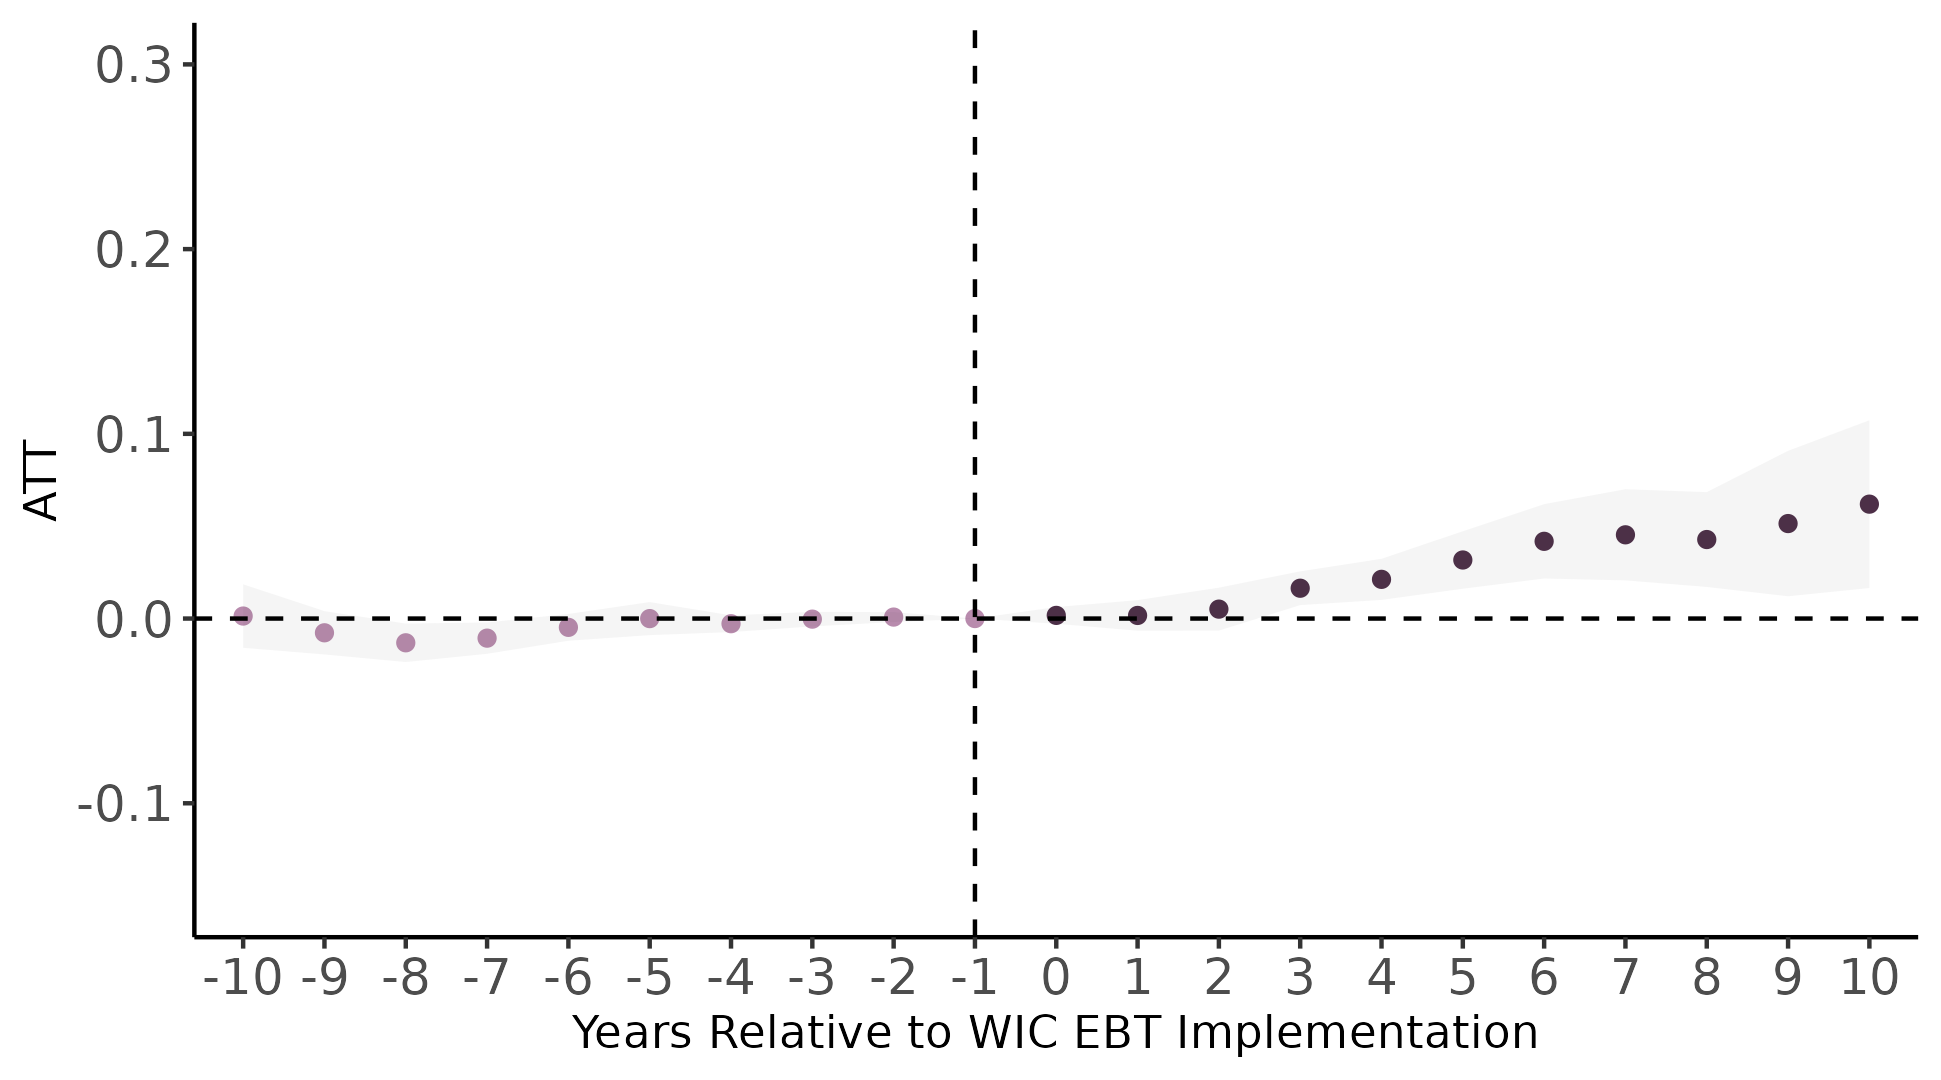
\includegraphics[width=\textwidth]{wic_br_dyn_all_noncov.png}  
		\caption{All births, without Controlling for County Baseline Characteristics}
		\label{cs_es1}
	\end{subfigure}
	\begin{subfigure}[t]{.325\textwidth}
		\centering
		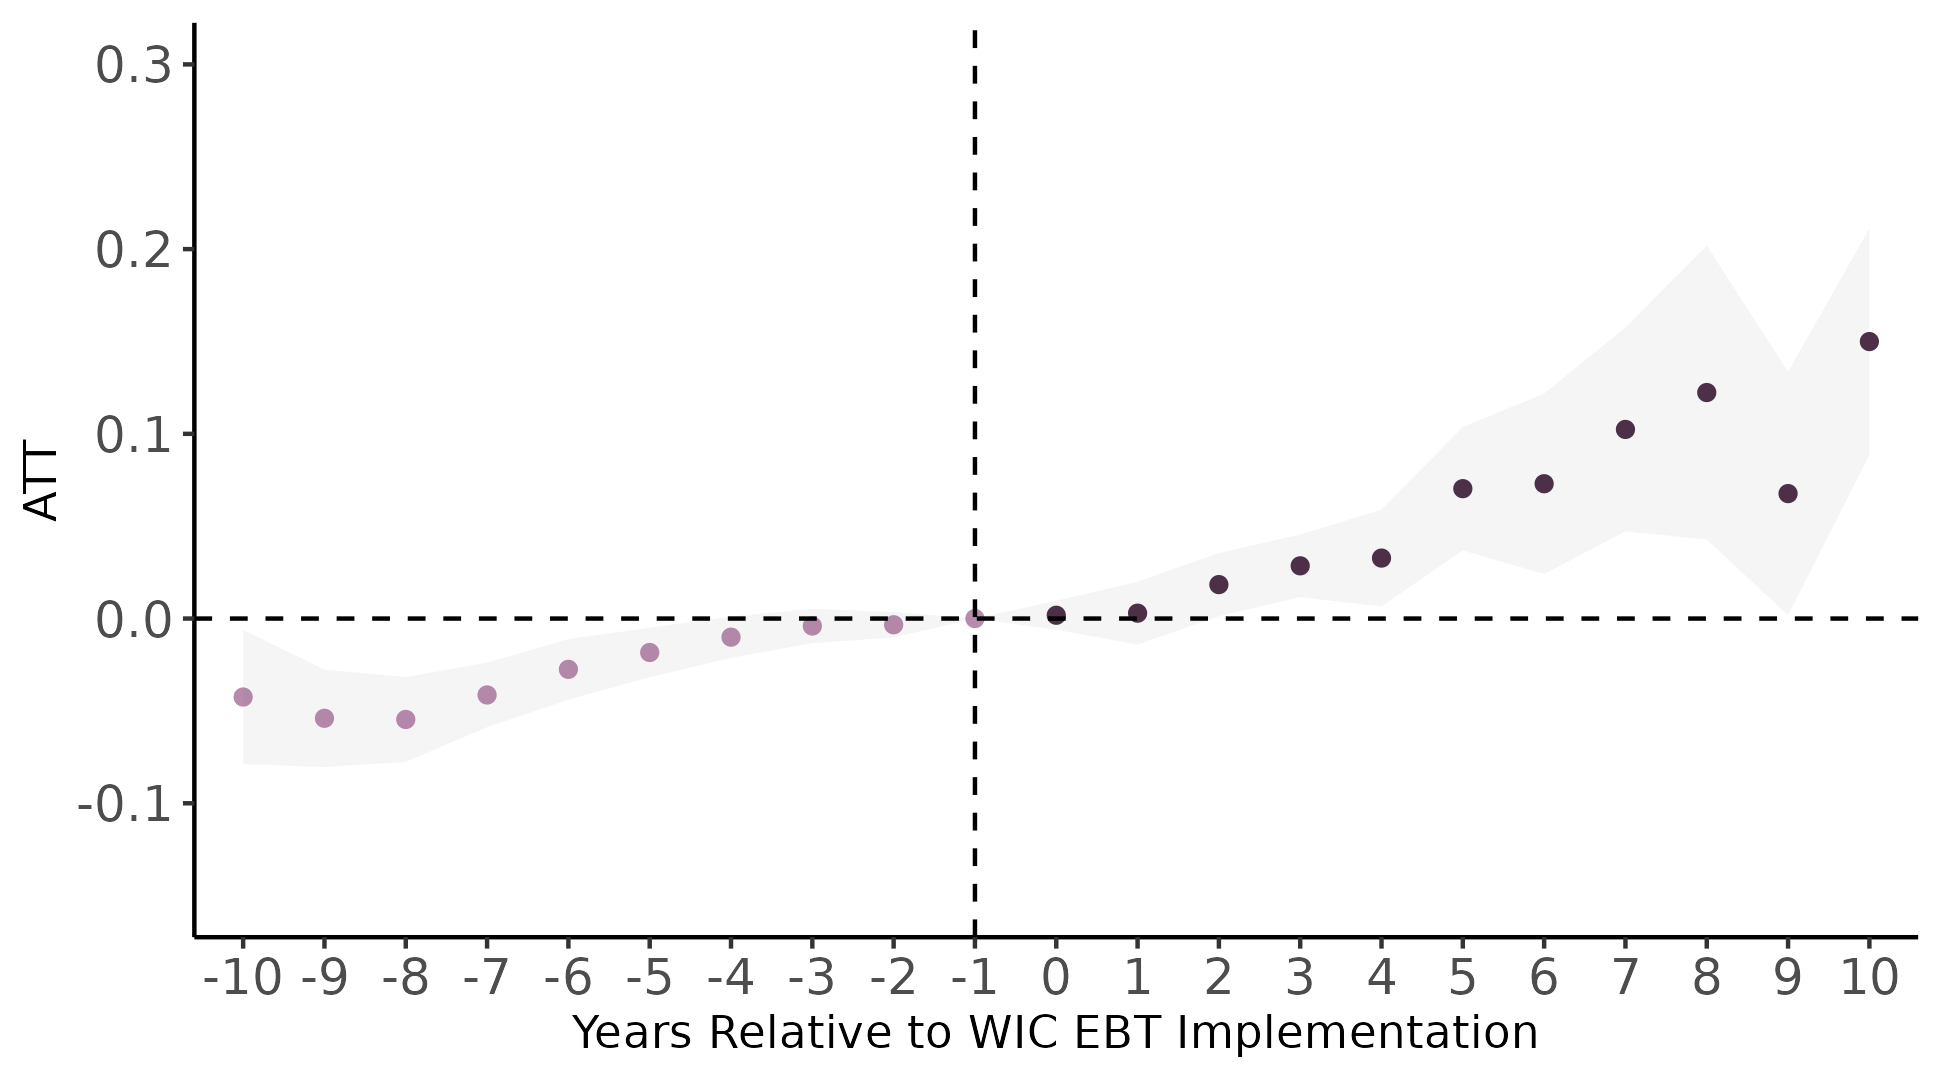
\includegraphics[width=\textwidth]{wic_br_dyn_leum_noncov.png}  
		\caption{LEUM Births, without Controlling for County Baseline Characteristics}
		\label{cs_es2}
	\end{subfigure}
	\begin{subfigure}[t]{.325\textwidth}
		\centering
		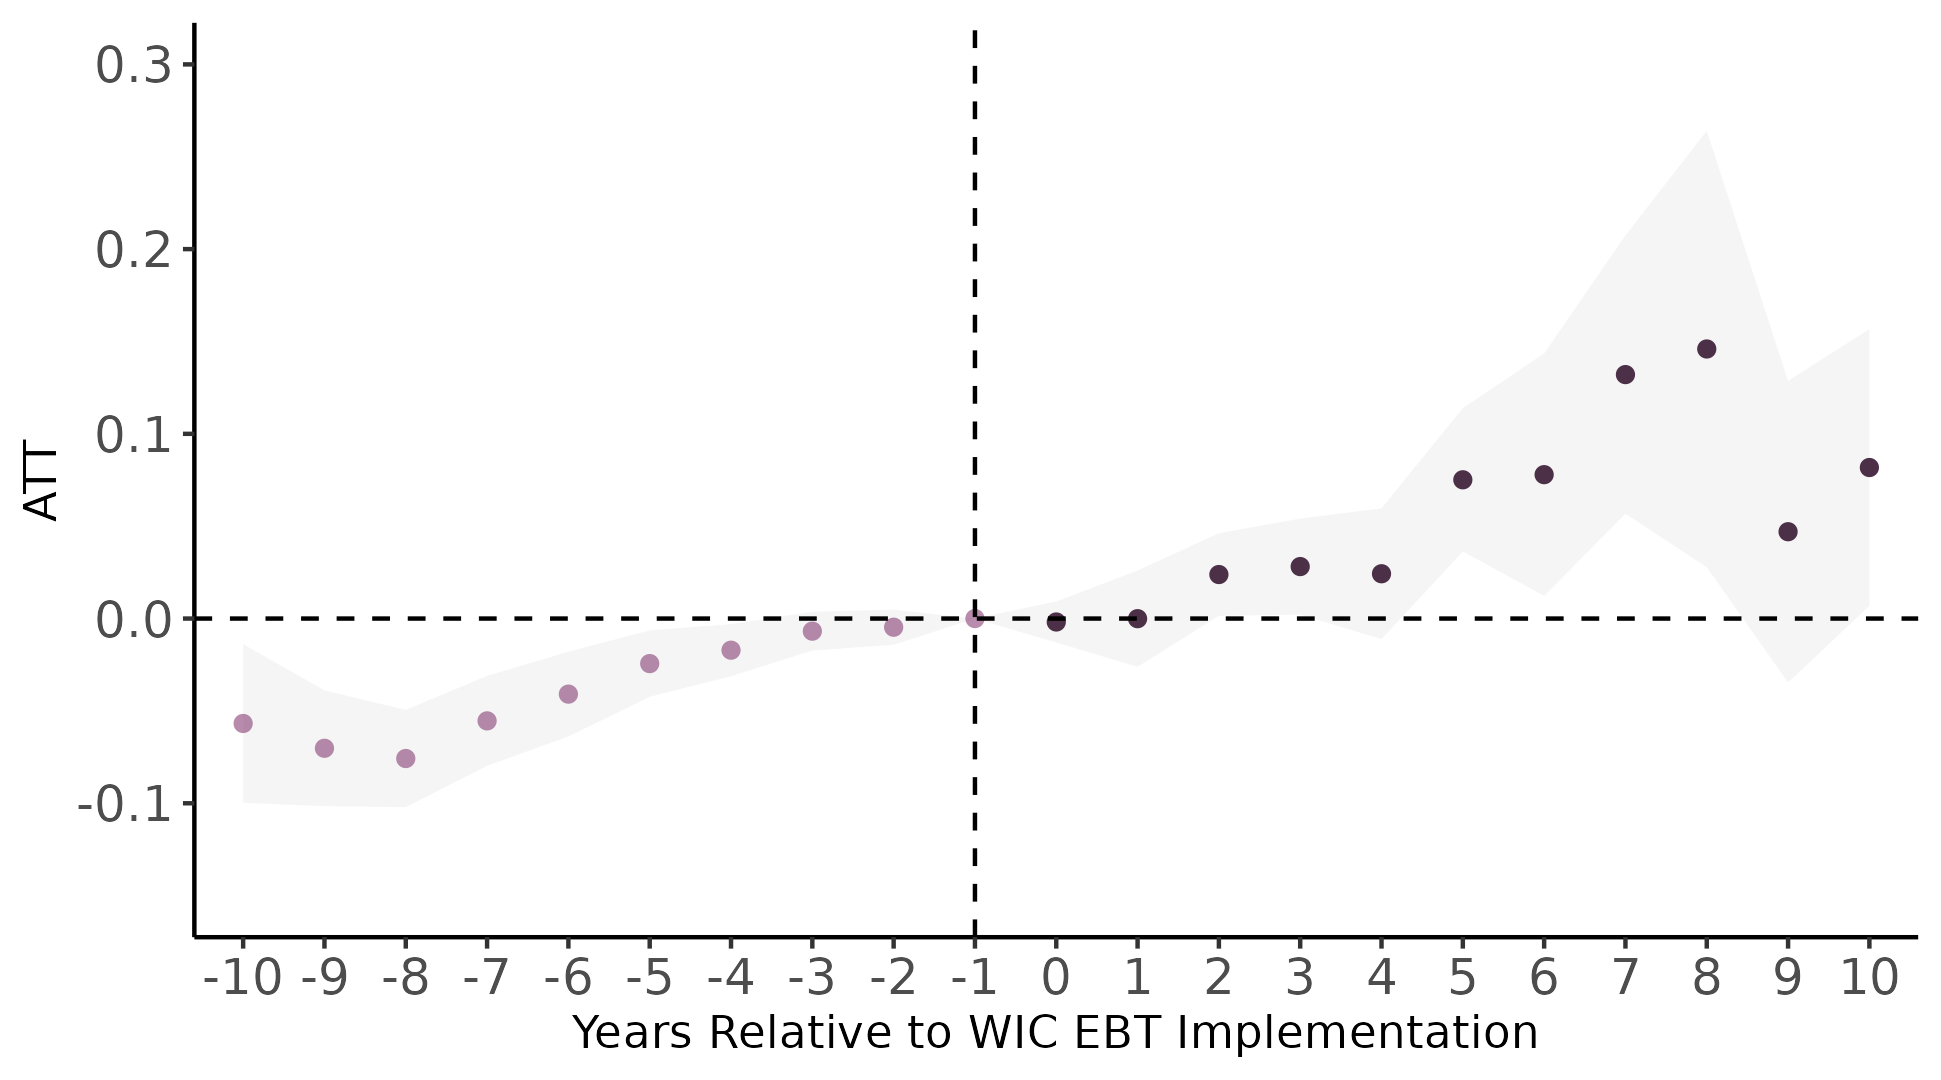
\includegraphics[width=\textwidth]{wic_br_dyn_leum_minor_noncov.png}  
		\caption{LEUM $\times$ Black/Hispanic, without Controlling for County Baseline Characteristics}
		\label{cs_es3}
	\end{subfigure}
	\begin{subfigure}[t]{.325\textwidth}
		\centering
		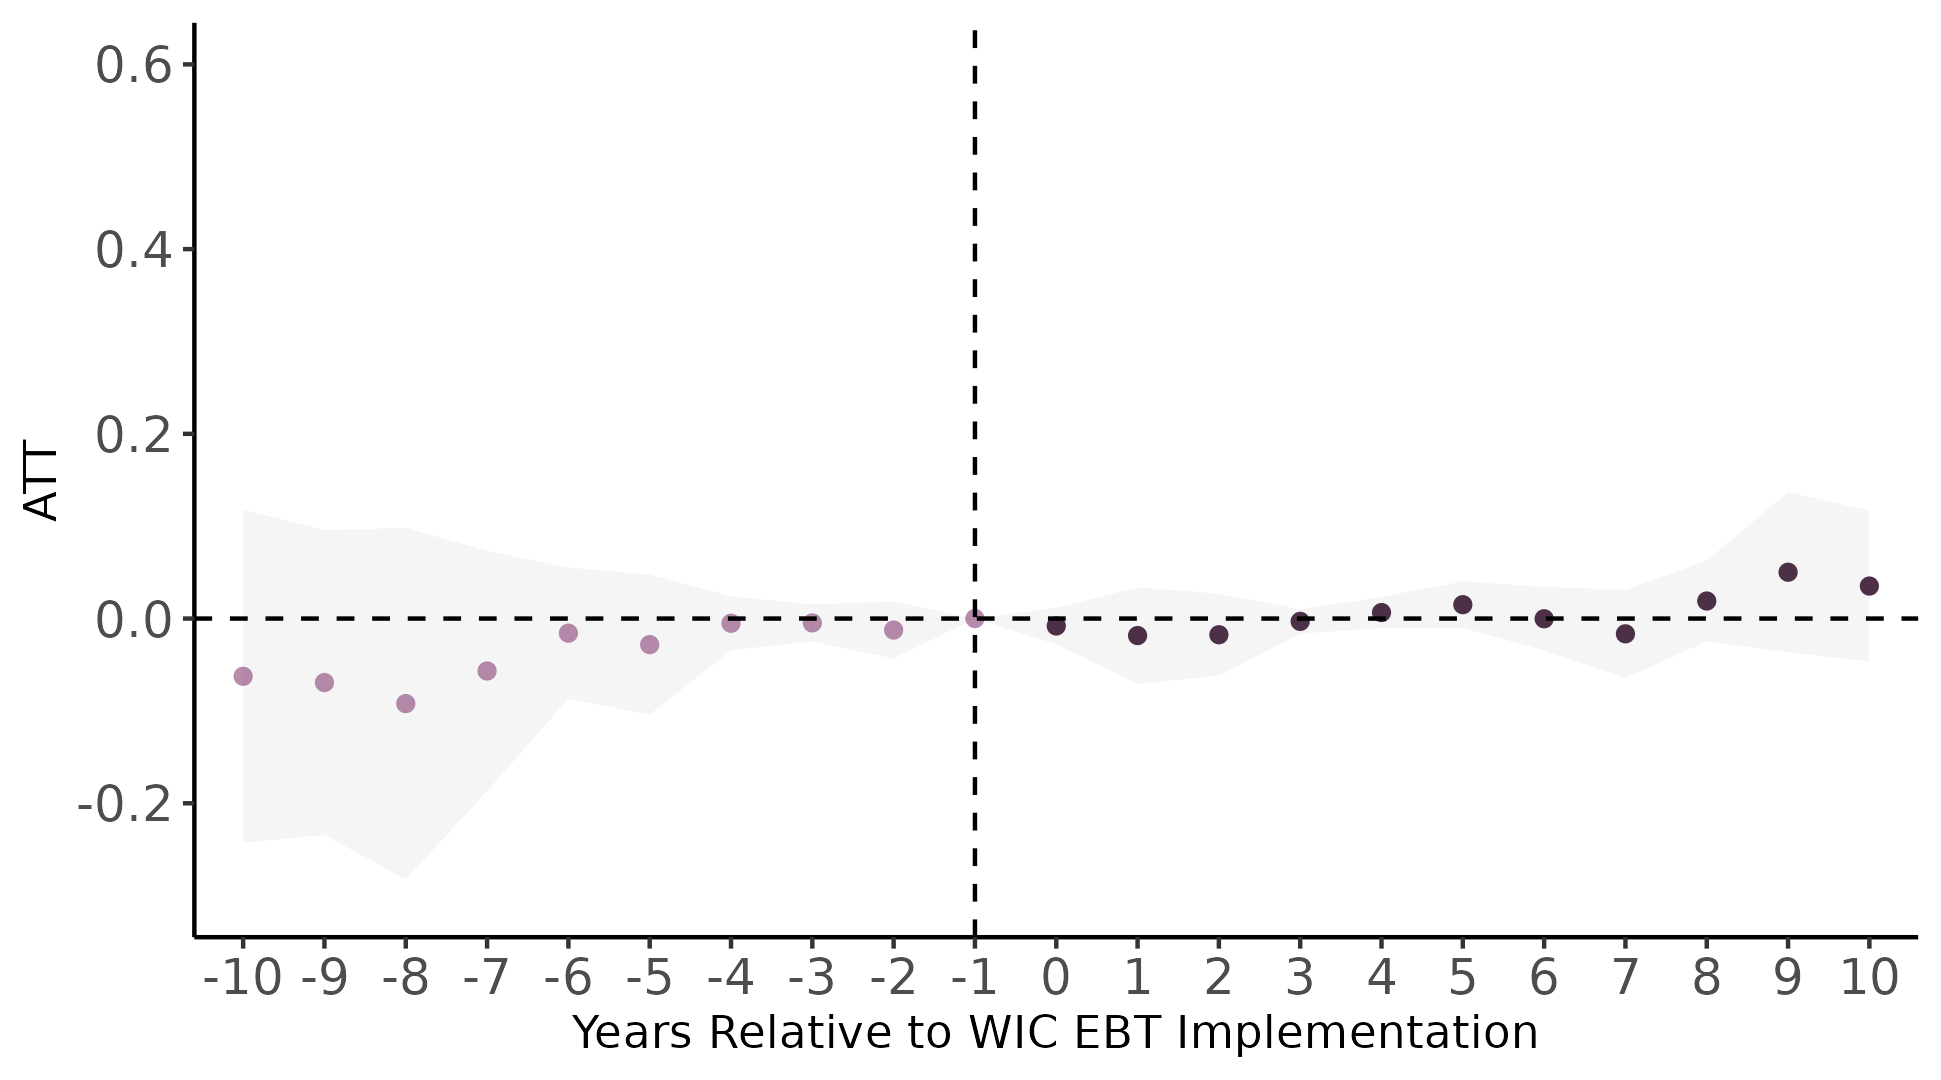
\includegraphics[width=\textwidth]{wic_br_dyn_all.png}  
		\caption{All Births, with Controlling for County Baseline Characteristics}
		\label{cs_es1}
	\end{subfigure}
	\begin{subfigure}[t]{.325\textwidth}
		\centering
		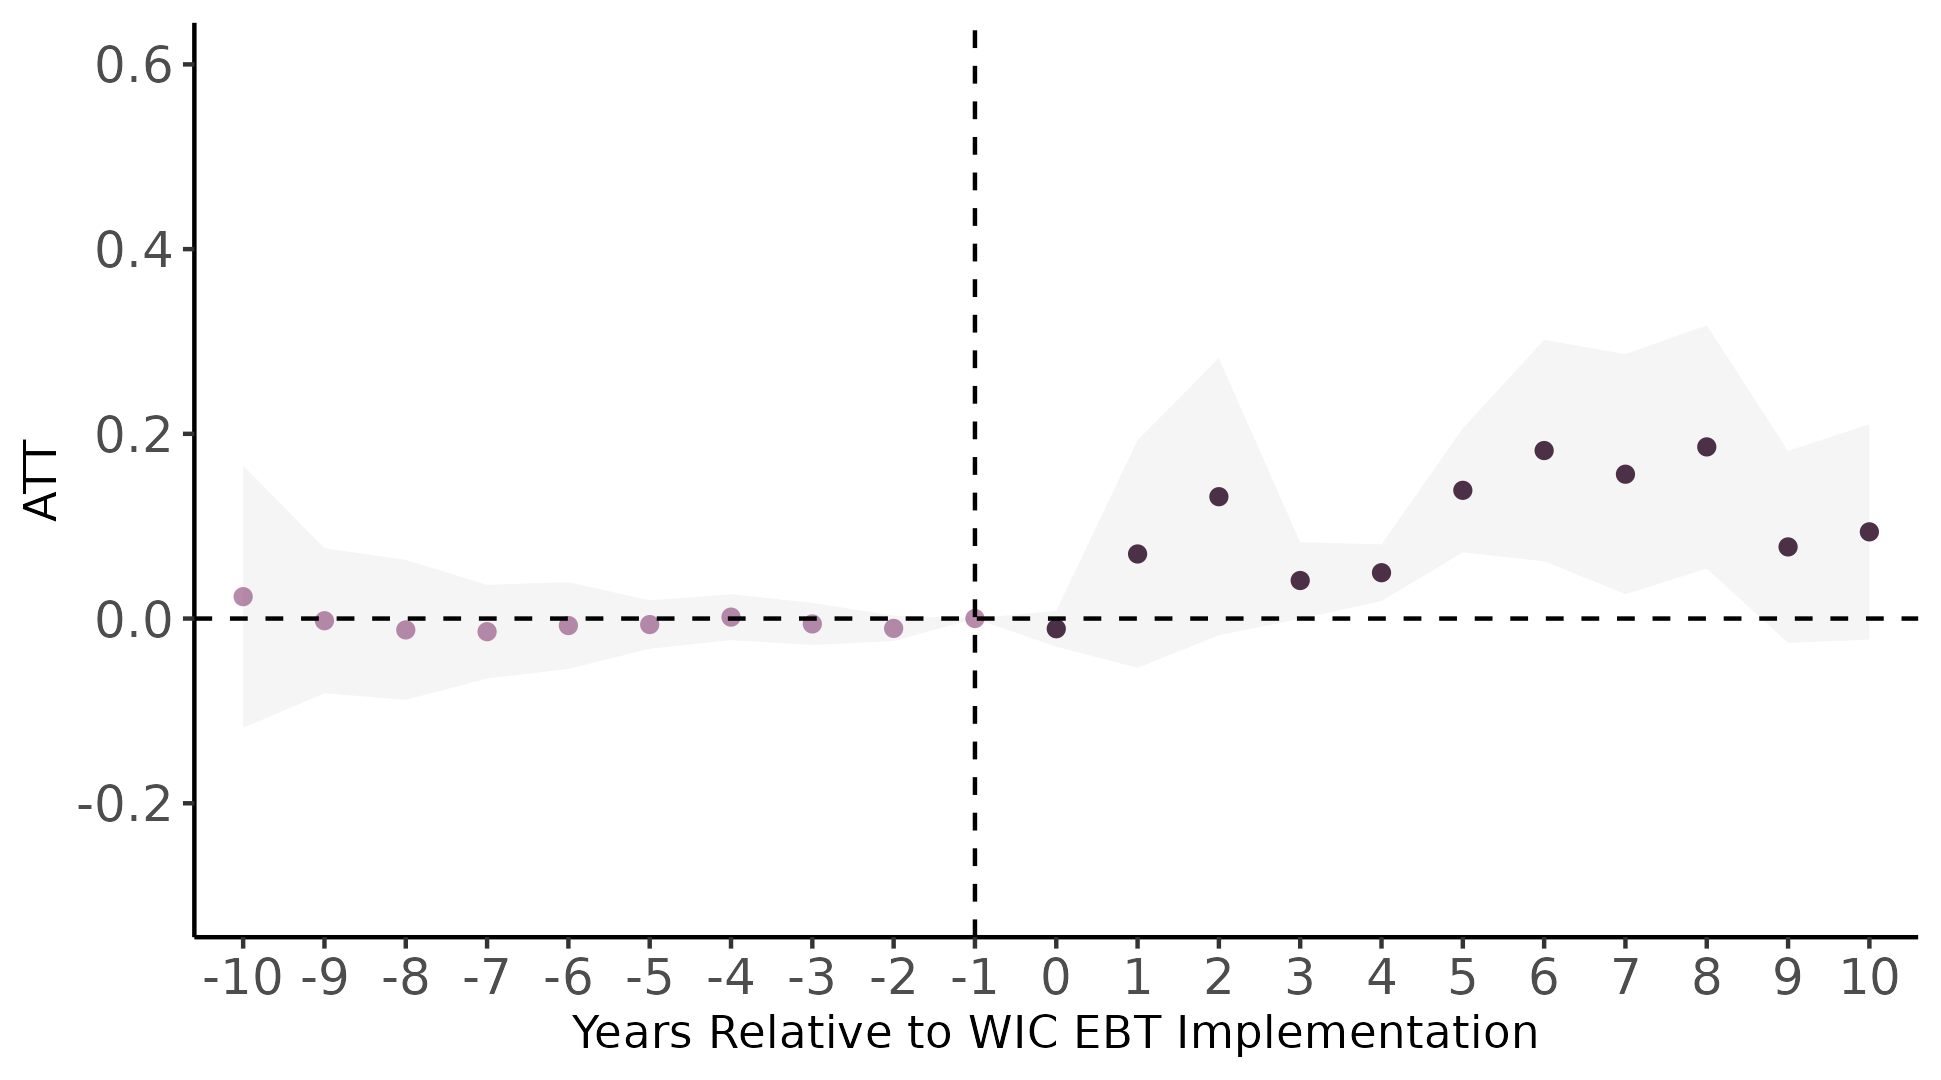
\includegraphics[width=\textwidth]{wic_br_dyn_leum.png}  
		\caption{LEUM Births, with Controlling for County Baseline Characteristics}
		\label{cs_es2}
	\end{subfigure}
	\begin{subfigure}[t]{.325\textwidth}
		\centering
		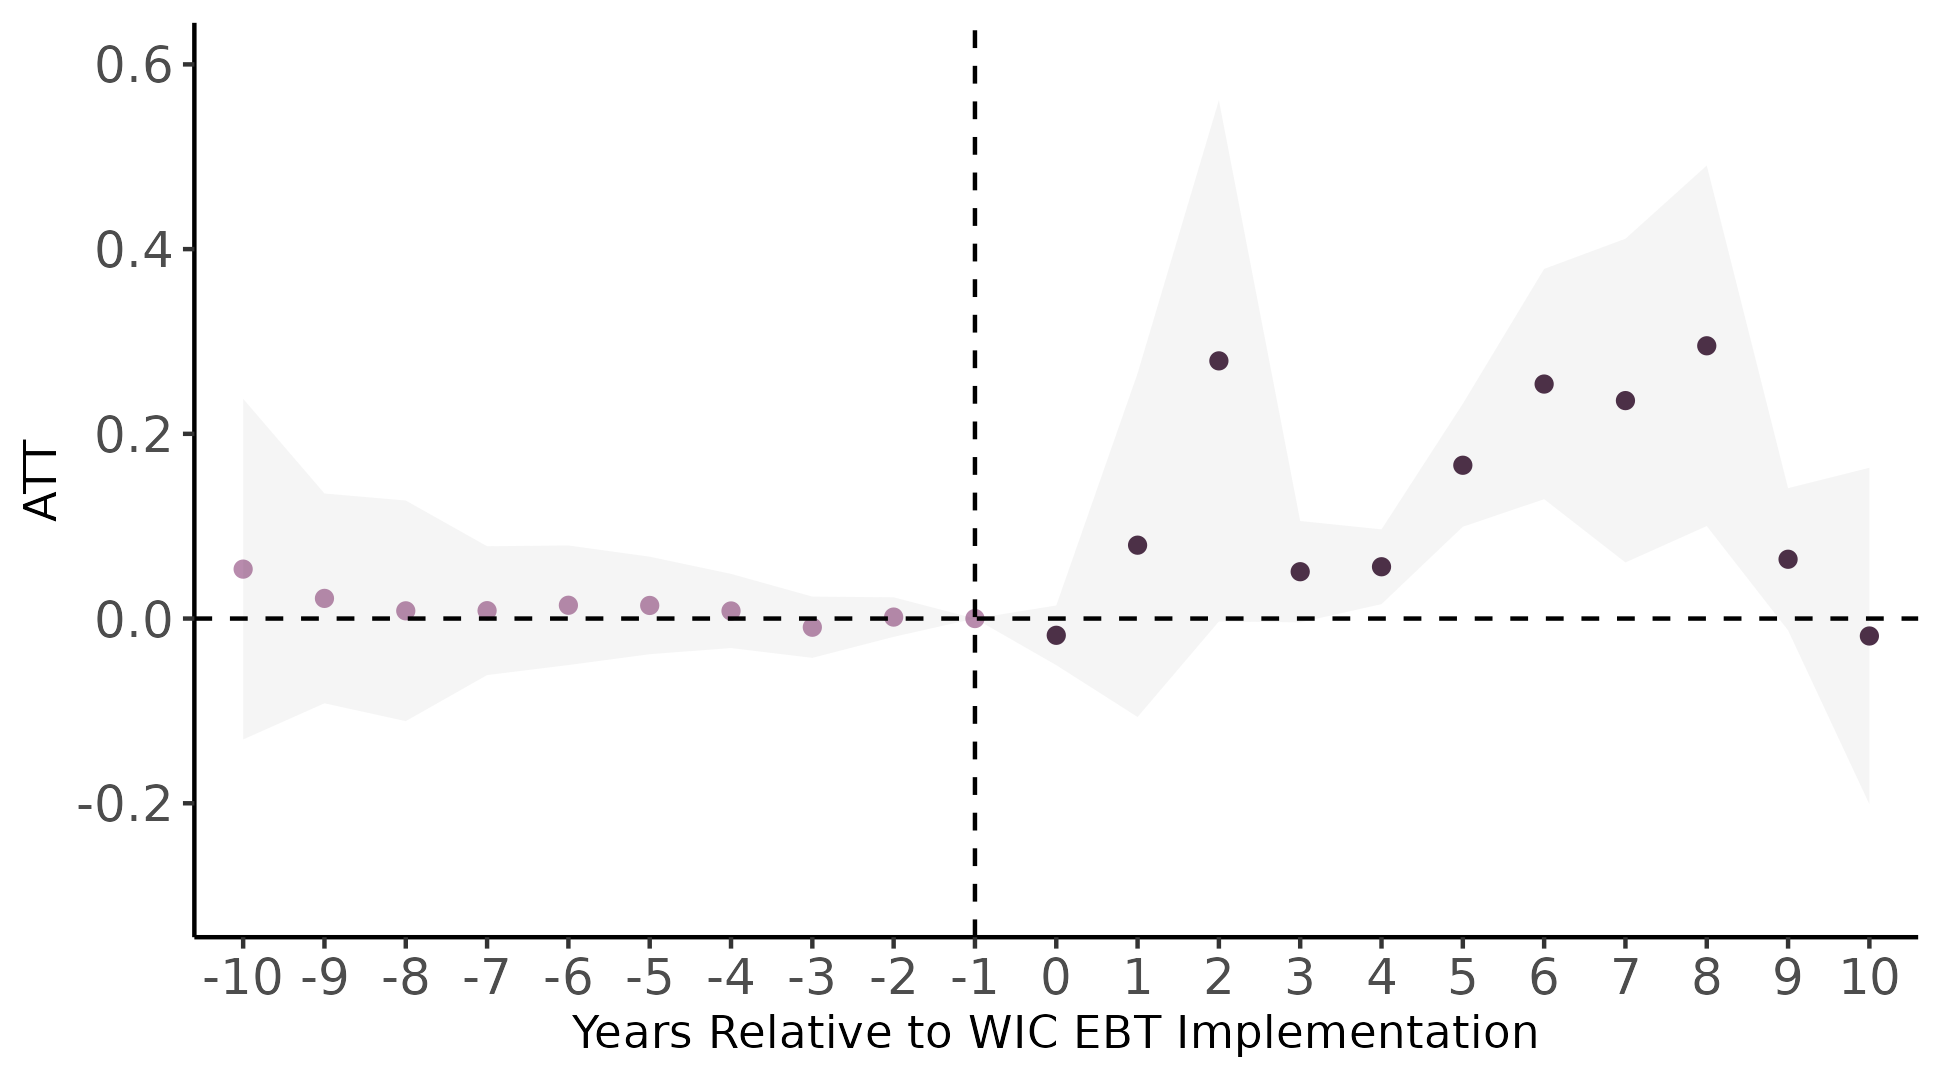
\includegraphics[width=\textwidth]{wic_br_dyn_leum_minor.png}  
		\caption{LEUM $\times$ Black/Hispanic, with Controlling for County Baseline Characteristics}
		\label{cs_es3}
	\end{subfigure}
	\caption{\textsc{Dynamic Effects of WIC EBT on Share of WIC Births}}
	\label{cs_es}
	\footnotesize
	\vspace{6pt}
	\vspace{4pt}
	Notes: LEUM refers to births given by unmarried mothers with less than high school education. Regressions are weighted by the number of births of cells. Standard errors are clustered at the county level. We use not-yet-treated counties as comparison group. We drop cells with fewer than 25 births.
\end{figure}

\begin{figure}
	\begin{center}
		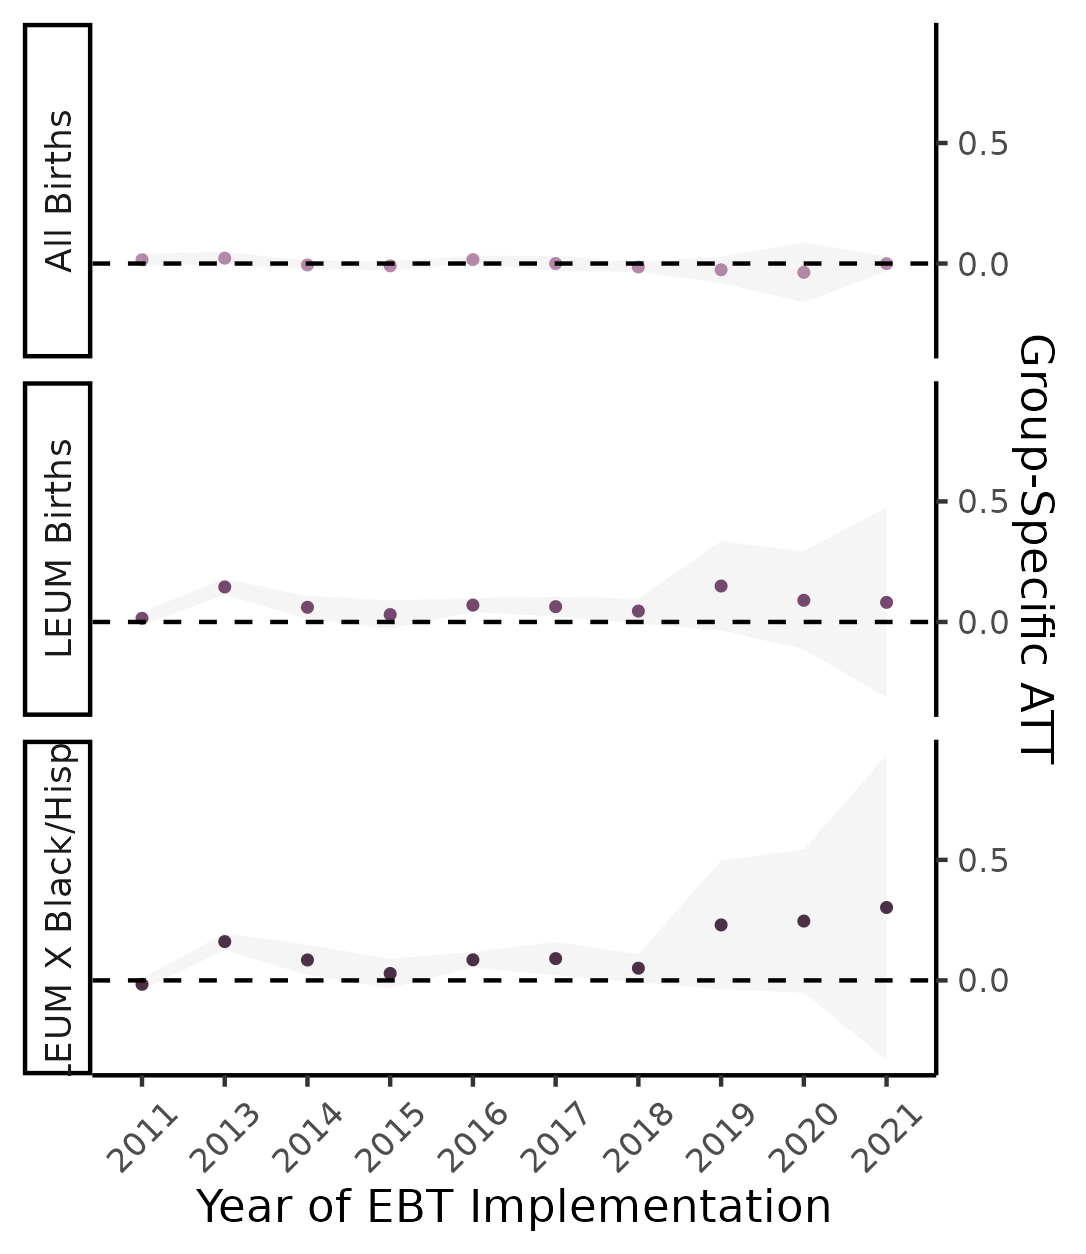
\includegraphics[width=.6\textwidth]{group_att.png}  
		\caption{\textsc{Group-specific Effects of WIC EBT on WIC Birth Ratio}}
		\label{group_att}
	\end{center}
	\footnotesize
	Notes: 
\end{figure}

\section{Robustness}

\begin{table}[!htbp]
	\begin{center}
		\caption{\textsc{Sensitivity to Sample Selection}} 
		\label{} 
		\scriptsize
		\begin{tabularx}{\linewidth}{@{}l*{9}{>{\centering\arraybackslash}X}@{}}
			\\[-1.8ex]\hline 
			\hline 
			\\[-1.8ex] 
			& \multicolumn{9}{c}{WIC Birth Ratio} \\ 
			\cline{2-10} \\
			& \multicolumn{3}{c}{All} & \multicolumn{3}{c}{LEUM} & \multicolumn{3}{c}{LEUM $\times$ Black/Hisp.} \\
			\cmidrule(lr){2-4}\cmidrule(lr){5-7} \cmidrule(lr){8-10}
			& Full    & $\geq 15$     & $\geq 35$     & Full    & $\geq 15$     & $\geq 35$    & Full    & $\geq 15$     & $\geq 35$     \\
			[1ex]            & (1)     & (2)      & (3)    & (4)  & (5)     & (6)      & (7)    & (8) & (9)    \\
			\midrule
			Born after EBT  & -0.0077 & -0.0167 & -0.0143 & 0.0447 & 0.0853$^{**}$  &0.1085$^{**}$ & 0.0152 & 0.1378$^{**}$  & 0.1673$^{**}$ \\
			& (0.0167) & (0.0198) & (0.0226) & (0.0317) & (0.0380) & (0.0475) & (0.0569) & (0.0515) & (0.1113)\\  \\
			Covariates     & \checkmark & \checkmark & \checkmark & \checkmark & \checkmark & \checkmark
			& \checkmark & \checkmark & \checkmark  \\
			Observations    & 28,756 & 22,438 & 19,955 & 19,864 & 10,153 & 6,110 & 11,466 & 4,420  & 3,016\\
			Dep. Var. Mean (DVM) & 0.4215 & 0.4261 & 0.4358 & 0.7393 & 0.7390 & 0.7319 & 0.7482 & 0.7440 & 0.7366\\
			\%(ATT/DVM) & 1.83\% & 3.92\% & 3.28\% & 6.05\% & 12.65\% & 14.82\% & 2.03\% & 18.52\% & 22.71\%\\
			\hline \\[-1.8ex] 
			\hline 
			\hline \\ [-5.0ex] 		
		\end{tabularx}
	\end{center}
	\footnotesize
	\vspace{4pt}
	Notes: 
\end{table}

\begin{table}[!htbp] 
	\begin{center}
		\caption{\textsc{Two-way-fixed-effect Estimators and Goodman-Bacon Decomposition}} 
		\label{twfe} 
		\scriptsize 
		\begin{tabularx}{.75\linewidth}{@{}l*{3}{>{\centering\arraybackslash}X}@{}}
			\\[-1.8ex]\hline 
			\hline 
			\\[-1.8ex] 
			& \multicolumn{3}{c}{WIC Birth Ratio} \\ 
			\cline{2-4}   
			\\[-1.8ex] & All Births   & LUEM Births & LUEM $\times$ Black/Hisp.  \\ 
			\\[-1.8ex] & \multicolumn{1}{c}{(1)} & \multicolumn{1}{c}{(2)}  & \multicolumn{1}{c}{(3)} \\ 
			\hline \\[-1.8ex] 
			TWFE Est. &  0.0071$^{***}$  & 0.0099$^{***}$ & 0.0094$^{**}$  \\
			& (0.0013)& (0.0028) & (0.0043) \\ 
			TWFE Est., No Forbidden Comparison &  	
			0.0094 & 0.0181 & 0.0167 \\
			$\Delta$ after excl. the Forbidden Comparison &  	
			$\uparrow$ 32.39\% & $\uparrow$ 82.83\% &  $\uparrow$ 77.66\% \\
			& & & \\
			County FE & \checkmark & \checkmark & \checkmark \\
			Year FE & \checkmark & \checkmark & \checkmark  \\
			Observations & 18,824 & 7,709 & 3,549 \\
			Dep. Var. Mean & 0.4212 & 0.7363 & 0.7415 \\
			\hline \\[-1.8ex] 
			\hline 
			\hline \\ [-5.0ex] 
		\end{tabularx} 
	\end{center}
	\footnotesize
	Note: We use the same balanced panel as CS estimators. Goodman-Bacon decomposition can only work on balanced panels and can only identify the forbidden comparison (the later v.s. earlier group) for the case without any controls \citep{goodman2021difference}.
\end{table} 

\begin{table}[!htbp] 
	\begin{center}
		\caption{\textsc{Alternative Staggered DD Estimators}} 
		\label{sa} 
		\footnotesize 
		\begin{tabularx}{.9\linewidth}{@{}l*{6}{>{\centering\arraybackslash}X}@{}}
			\\[-1.8ex]\hline 
			\hline 
			\\[-1.8ex] 
			& \multicolumn{3}{c}{CS 2020} & \multicolumn{3}{c}{SA 2021}\\ 
			& \multicolumn{3}{c}{Last-treated as Comparison} & \multicolumn{3}{c}{}\\ 
			\cmidrule(lr){2-4}\cmidrule(lr){5-7} 
			& All Births & LEUM Births & LEUM $\times$ Black/Hisp. & All Births & LEUM Births & LEUM $\times$ Black/Hisp.\\ 
			\\[-1.8ex] & \multicolumn{1}{c}{(1)} & \multicolumn{1}{c}{(2)}& \multicolumn{1}{c}{(3)} & \multicolumn{1}{c}{(4)} & \multicolumn{1}{c}{(5)}& \multicolumn{1}{c}{(6)} \\ 
			\hline \\[-1.8ex] 
			Born after EBT   & -0.0269 & 0.1415$^{**}$ &0.1895$^{***}$ & 0.0078 & 0.0246$^{**}$ & 0.0256$^{**}$ \\
			& (0.0256) & (0.0614) &(0.0936) & (0.0054) &(0.0109) & (0.0141) \\
			& & & & & & \\
			Covariates  & \checkmark & \checkmark & \checkmark & \checkmark & \checkmark & \checkmark \\
			Observations    & 20,956 & 7,709 & 3,549 & 20,955 &7,708 & 3,548 \\
			Dep. Var. Mean   & 0.4321 & 0.7363 & 0.7415 & 0.4321 &0.7363 & 0.7415 \\
			\%(ATT/DVM)  & -6.23\% & 19.22\% & 25.56\% & 1.81\% & 3.34\% & 3.32\% \\
			\hline \\[-1.8ex] 
			\hline 
			\hline \\ [-5.0ex] 
		\end{tabularx}
	\end{center}
	\footnotesize
	\vspace{4pt}
	Notes: SA 2021 estimators are from \cite{sun2021estimating}.
\end{table} 


\begin{table}[!htbp] 
	\begin{center}
		\caption{\textsc{Alternative Definitions of Likely Eligible Sub-population}} 
		\label{sa} 
		\footnotesize 
		\begin{tabularx}{\linewidth}{@{}l*{6}{>{\centering\arraybackslash}X}@{}}
			\\[-1.8ex]\hline 
			\hline 
			\\[-1.8ex] 
			& Age $\leq$ 22 & Education $<$ HS & Unmarried & Black/Hispanic & LEUM Births & LEUM $\times$ Black/Hisp.\\ 
			\\[-1.8ex] & \multicolumn{1}{c}{(1)} & \multicolumn{1}{c}{(2)}& \multicolumn{1}{c}{(3)} & \multicolumn{1}{c}{(4)} & \multicolumn{1}{c}{(5)}& \multicolumn{1}{c}{(6)} \\ 
			\hline \\[-1.8ex] 
			Born after EBT   & -0.0269 & 0.1415$^{**}$ &0.1895$^{***}$ & 0.0078 & 0.0246$^{**}$ & 0.0256$^{**}$ \\
			& (0.0256) & (0.0614) &(0.0936) & (0.0054) &(0.0109) & (0.0141) \\
			& & & & & & \\
			Covariates  & \checkmark & \checkmark & \checkmark & \checkmark & \checkmark & \checkmark \\
			Observations    & 20,956 & 7,709 & 3,549 & 20,955 &7,708 & 3,548 \\
			Dep. Var. Mean   & 0.4321 & 0.7363 & 0.7415 & 0.4321 &0.7363 & 0.7415 \\
			\%(ATT/DVM)  & -6.23\% & 19.22\% & 25.56\% & 1.81\% & 3.34\% & 3.32\% \\
			\hline \\[-1.8ex] 
			\hline 
			\hline \\ [-5.0ex] 
		\end{tabularx}
	\end{center}
	\footnotesize
	\vspace{4pt}
	Notes: SA 2021 estimators are from \cite{sun2021estimating}.
\end{table} 


\begin{table}[!htbp] 
	\begin{center}
		\caption{\textsc{Composition Change}} 
		\label{sa} 
		\footnotesize 
		\begin{tabularx}{.6\linewidth}{@{}l*{2}{>{\centering\arraybackslash}X}@{}}
			\\[-1.8ex]\hline 
			\hline 
			\\[-1.8ex] & \multicolumn{1}{c}{Share of LEUM} & \multicolumn{1}{c}{Share of LEUM} \\
			& \multicolumn{1}{c}{Births} & \multicolumn{1}{c}{$\times$ Black/Hisp.} \\
			\\[-1.8ex] & \multicolumn{1}{c}{(1)} & \multicolumn{1}{c}{(2)}\\ 
			\hline \\[-1.8ex] 
			Born after EBT   & 0.0032 & 0.0062$^{*}$\\
			& (0.0037) & (0.0035)  \\
			& &  \\
			Covariates  &\checkmark & \checkmark  \\
			Observations   & 20,956 & 20,956  \\
			Dep. Var. Mean   & 0.0906 & 0.0319  \\
			\%(ATT/DVM)  & 3.53\% & 19.44\%  \\
			\hline \\[-1.8ex] 
			\hline 
			\hline \\ [-5.0ex] 
		\end{tabularx}
	\end{center}
	\footnotesize
	\vspace{4pt}
	Notes: LEUM births refer to the births of unmarried mothers who do not graduate from high school (LEUM: less educated and unmarried). Advantaged births are those given to high-school-graduated, married, white mothers. Standard errors of both estimators are clustered at the county level. We drop cells with fewer than 25 births. $^{***}$, $^{**}$, and $^{*}$ indicate that the estimates are significant at the 1\%, 5\%, and 10\% levels.
\end{table} 


\section{Comparison to \cite{meckel2020cure}}
Our estimates are more credible than \cite{meckel2020cure} for several reasons. First, her event study plots show clear pretend trends once we extend them to a larger window. Second, we find that impacts on WIC births per county pick up mostly trends of number of births. Finally, after controlling for pretend, our CS estimators using Texas DSHS data show that Texas are not too different from other states.

\begin{figure}[!htbp]
	\begin{subfigure}[t]{.5\textwidth}
		\centering
		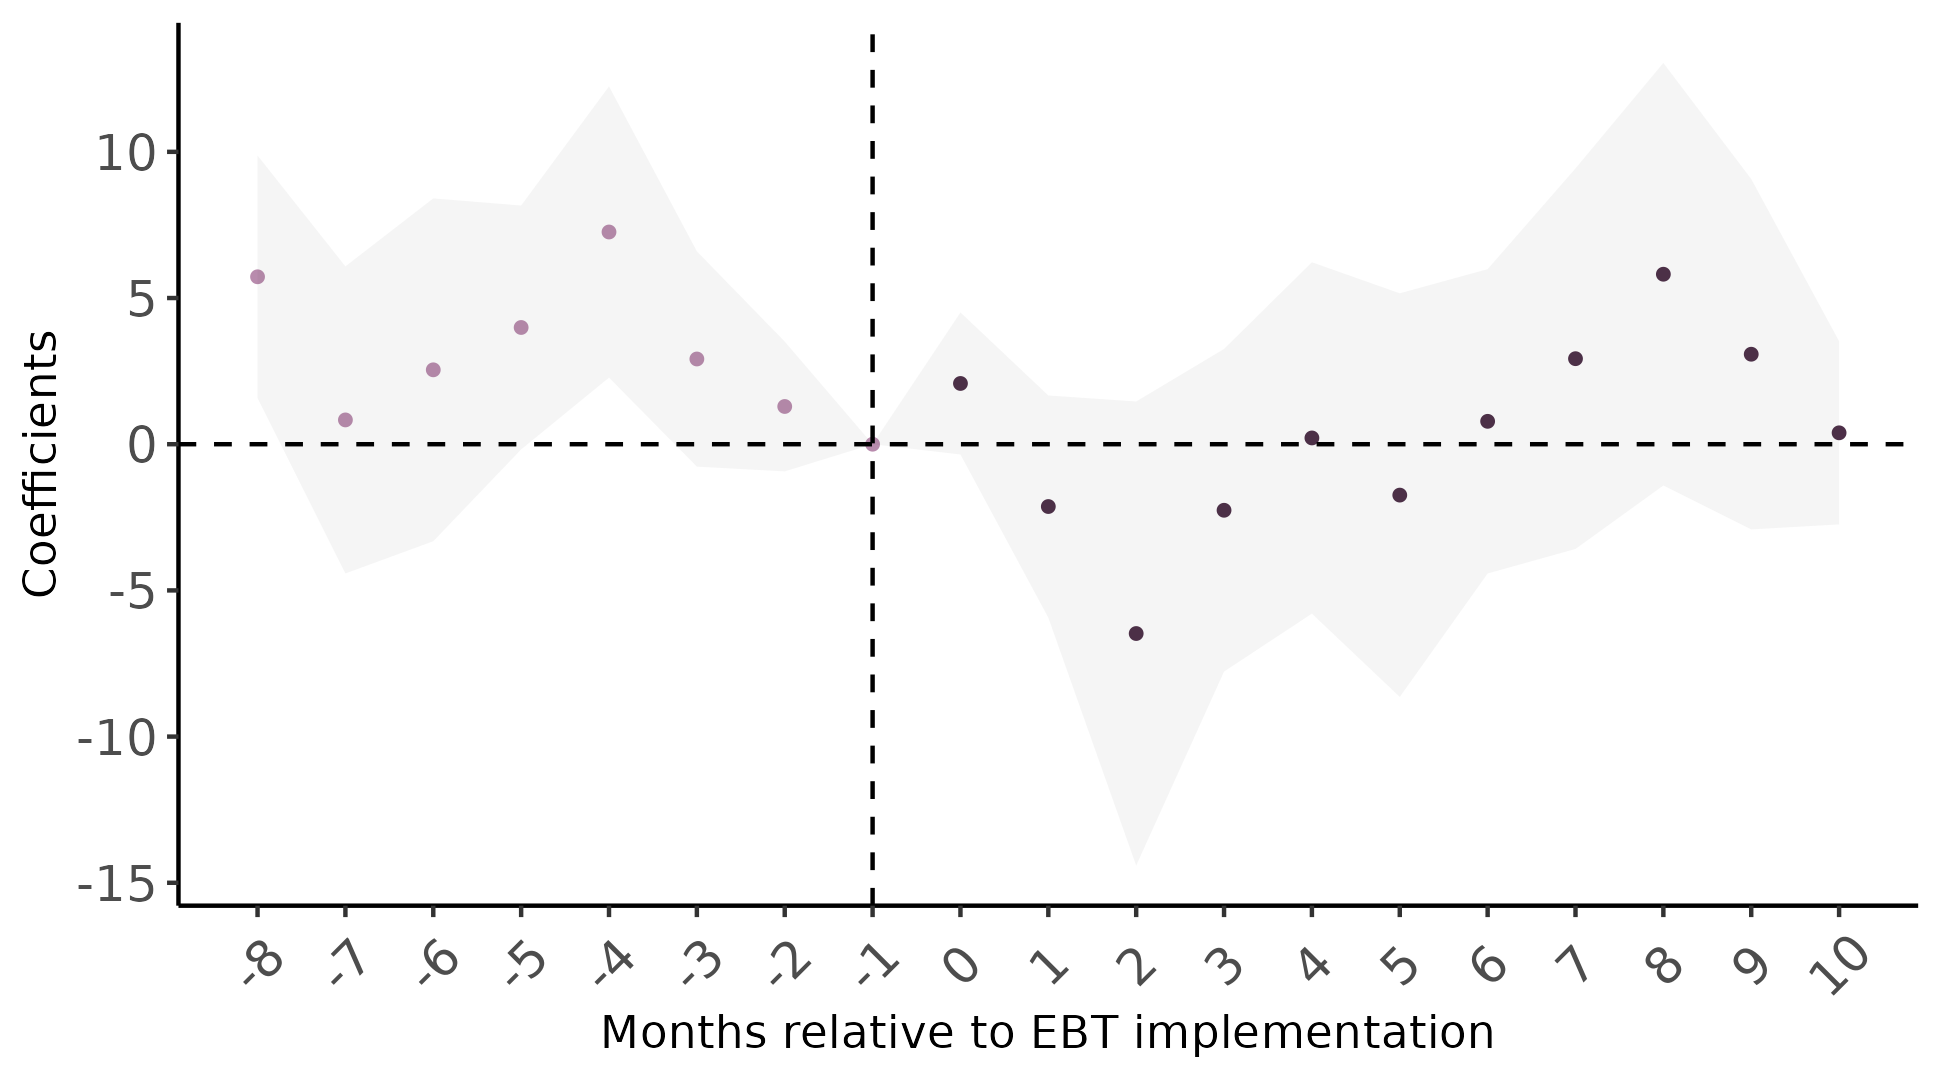
\includegraphics[width=\textwidth]{fig8_mk.png}  
		\caption{EBT and WIC Births per County (Figure 8 in \cite{meckel2020cure})}
		\label{mk_es1}
	\end{subfigure}
	\begin{subfigure}[t]{.5\textwidth}
		\centering
		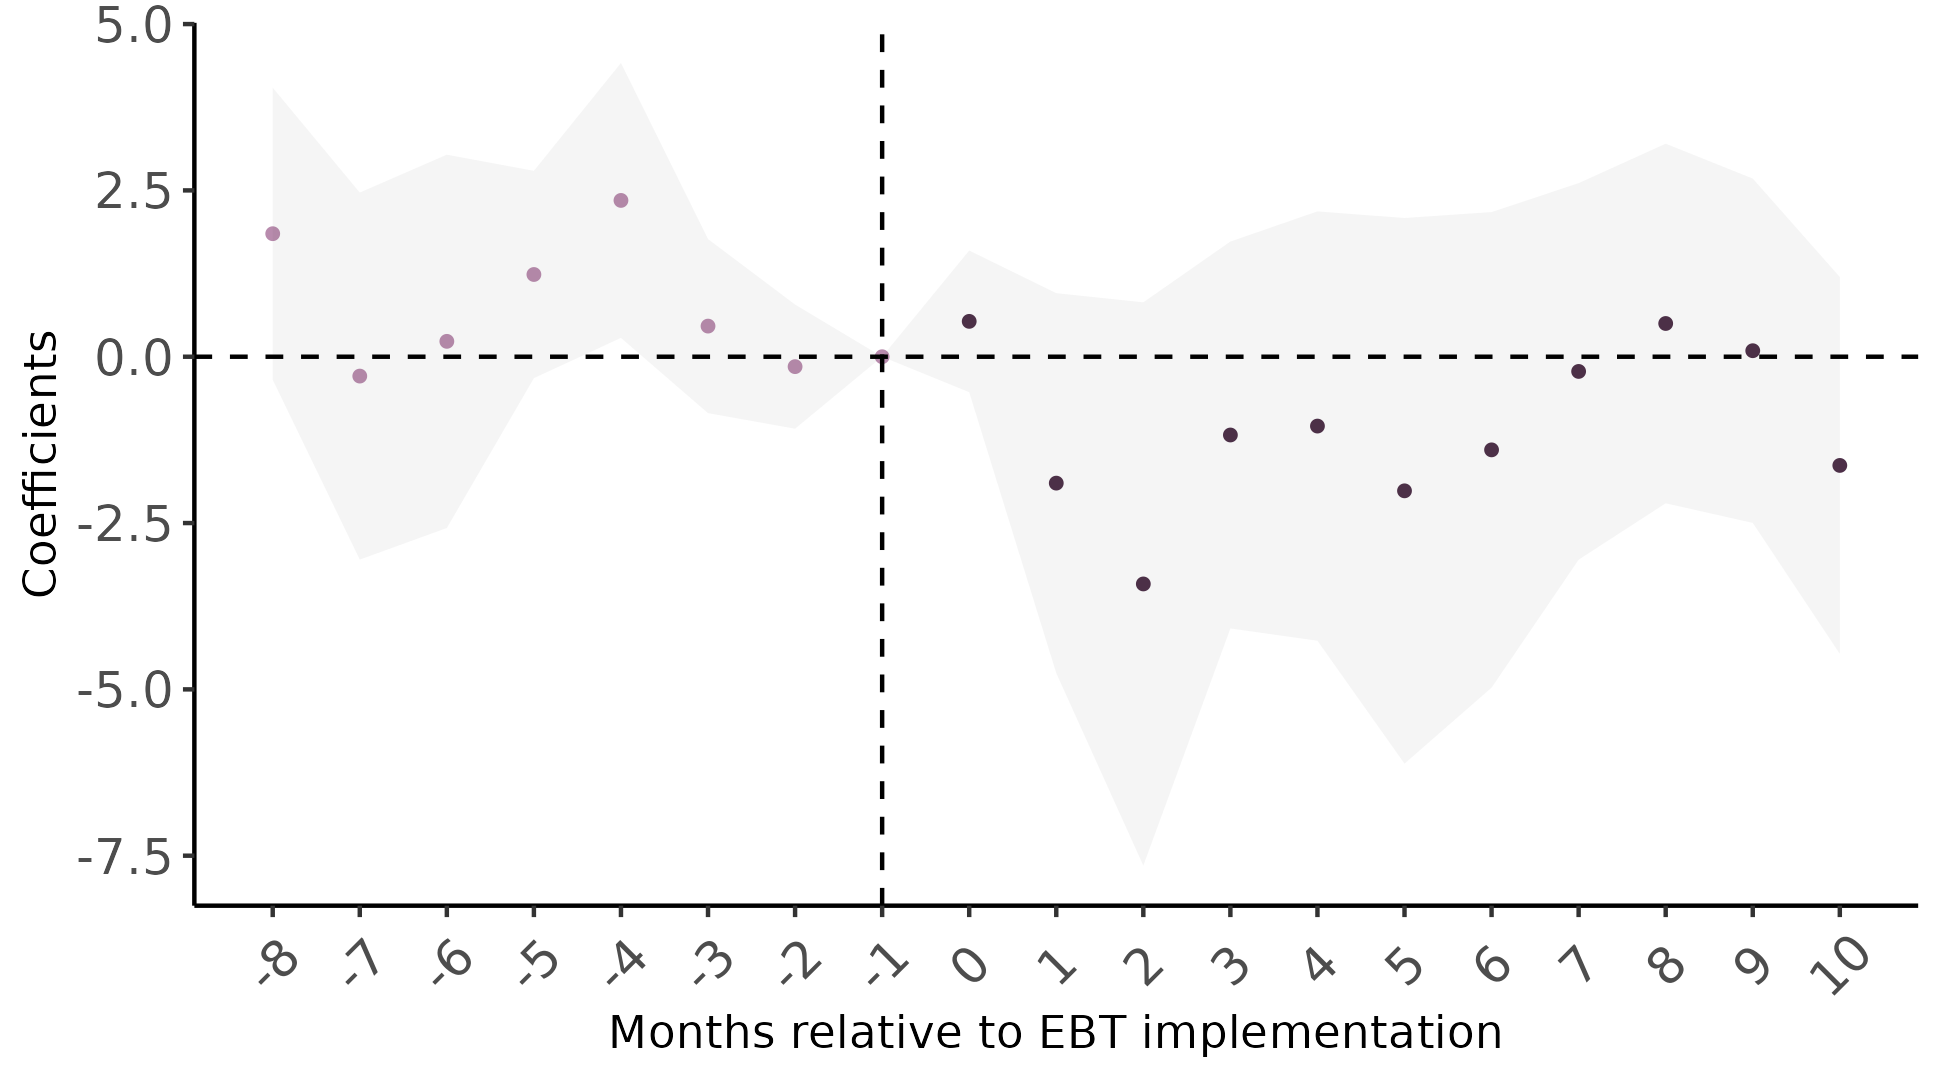
\includegraphics[width=\textwidth]{fig9_mk.png}  
		\caption{EBT and High Poverty WIC Births per County (Figure 8 in \cite{meckel2020cure})}
		\label{mk_es2}
	\end{subfigure}
	\begin{subfigure}[t]{.5\textwidth}
		\centering
		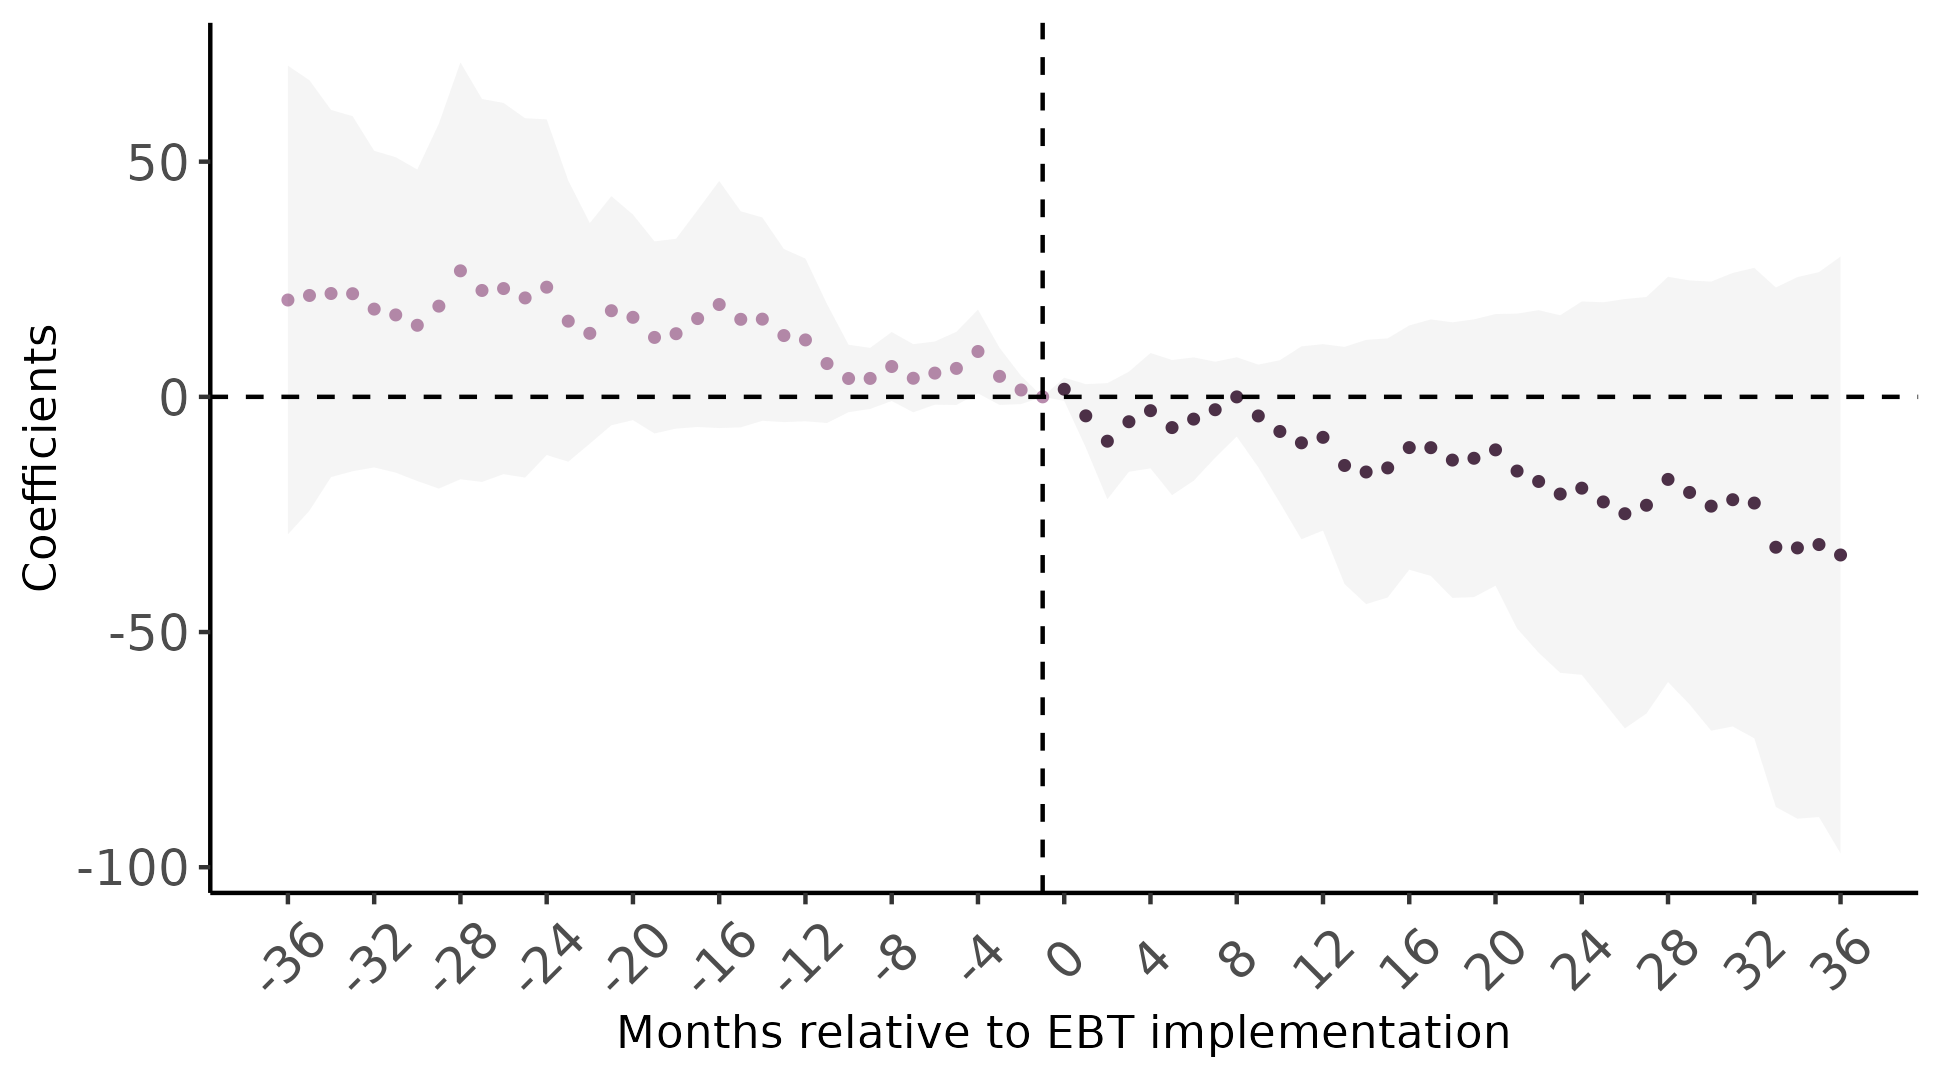
\includegraphics[width=\textwidth]{fig8_mk_long.png}  
		\caption{EBT and WIC Births per County, with A Larger Window}
		\label{mk_es3}
	\end{subfigure}
	\begin{subfigure}[t]{.5\textwidth}
		\centering
		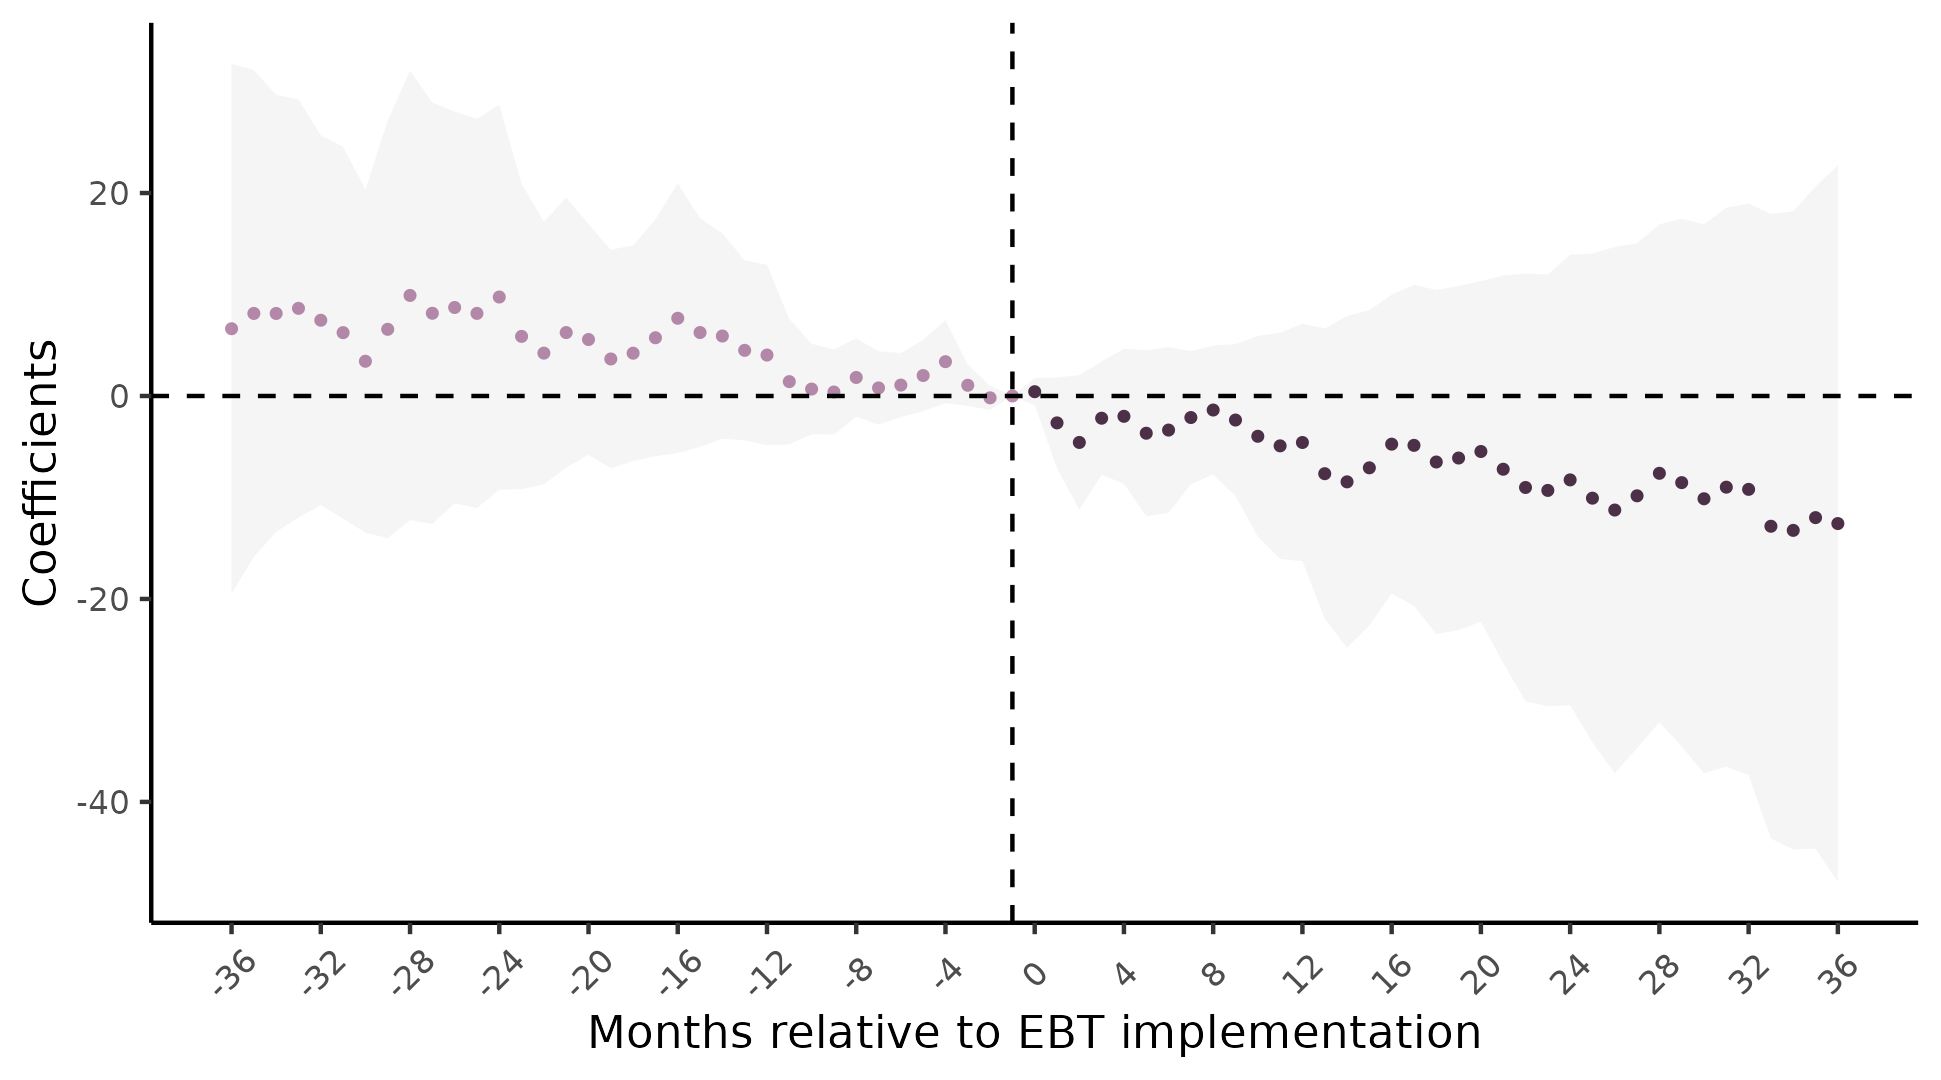
\includegraphics[width=\textwidth]{fig9_mk_long.png}  
		\caption{EBT and High Poverty WIC Births per County, with A Larger Window}
		\label{mk_es4}
	\end{subfigure}
	\caption{\textsc{Extending Event Study Plots in \cite{meckel2020cure} to A Larger Window}}
	\label{mk_es}
	\footnotesize
	\vspace{6pt}
	\vspace{4pt}
	Notes: 
\end{figure}


\begin{table}[!htbp]
	\begin{center}
		\caption{\textsc{Effects of EBT on WIC Births, Total Births, High Poverty Births, and High Poverty Births}} 
		\label{} 
		\scriptsize
		\begin{tabularx}{\linewidth}{@{}l*{8}{>{\centering\arraybackslash}X}@{}}
			\\[-1.8ex]\hline 
			\hline 
			\\[-1.8ex] 
			& \multicolumn{2}{c}{WIC Births} & \multicolumn{2}{c}{Total Births} & \multicolumn{2}{c}{High Poverty} & \multicolumn{2}{c}{High Poverty}  \\
			& \multicolumn{2}{c}{} & \multicolumn{2}{c}{} & \multicolumn{2}{c}{WIC Births} & \multicolumn{2}{c}{Births}  \\
			\cmidrule(lr){2-3}\cmidrule(lr){4-5} \cmidrule(lr){6-7}\cmidrule(lr){8-9}
			& (1)     & (2)      & (3)    & (4)  & (5)     & (6)      & (7)    & (8)    \\
			\midrule
			
			Born after EBT            & $-3.8563^{**}$ &                & $-3.9581^{**}$ &               & $-2.1681^{*}$ &                & $-1.9778^{**}$ &           \\
			& $(1.7398)$     &                & $(1.5992)$     &             & $(1.2410)$    &                & $(0.9566)$     &     \\
			Born 0-9 months &                & $-3.9151^{**}$ &                & $-3.7578^{**}$ &               & $-2.1380^{*}$  &                & $-1.9048^{**}$\\
			\hspace{8pt}    after EBT                       &                & $(1.8023)$     &                & $(1.5492)$     &               & $(1.2449)$     &                & $(0.9436)$    \\
			Born 10+ months  &                & $-3.2276^{**}$ &                & $-6.1000^{**}$  &               & $-2.4900^{**}$ &                & $-2.7591^{**}$ \\
			\hspace{8pt}    after EBT                &                & $(1.2863)$     &                & $(2.3564)$   &               & $(1.2604)$     &                & $(1.1791)$     \\
			\\
			R$^2$                     & $0.9893$       & $0.9893$       & $0.9961$       & $0.9961$    & $0.9854$      & $0.9854$       & $0.9923$       & $0.9923$     \\
			Observations                & $14,167$        & $14,167$        & $14,167$        & $14,167$    & $14,167$       & $14,167$        & $14,167$        & $14,167$      \\
			No. of Counties                & $239$          & $239$          & $239$          & $239$      & $239$         & $239$          & $239$          & $239$         \\  
			Dep. Var. Mean & $74.8541$ & $74.8541$ & $141.0398$ & $141.0398$ & $27.4343$ & $27.4343$ & $34.5791$ & $34.5791$  \\
			\hline \\[-1.8ex] 
			\hline 
			\hline \\ [-5.0ex] 		
		\end{tabularx}
	\end{center}
	\footnotesize
	\vspace{4pt}
	Notes: 
\end{table}

\begin{table}[!htbp]
	\begin{center}
		\caption{\textsc{Effects of EBT on WIC Birth Ratio and High Poverty WIC Birth Ratio}} 
		\label{} 
		\scriptsize
		\begin{tabularx}{.75\linewidth}{@{}l*{4}{>{\centering\arraybackslash}X}@{}}
			\\[-1.8ex]\hline 
			\hline 
			\\[-1.8ex] 
			& \multicolumn{2}{c}{WIC Birth Ratio} & \multicolumn{2}{c}{High Poverty} \\
			& \multicolumn{2}{c}{} & \multicolumn{2}{c}{WIC Birth Ratio} \\
			\cmidrule(lr){2-3}\cmidrule(lr){4-5}
			& (1)     & (2)      & (3)    & (4)    \\
			\midrule
			
			Born after EBT            & $-0.0153^{***}$ &                 & $-0.0218^{**}$ &                \\
			& $(0.0047)$      &                 & $(0.0088)$     &                \\
			Born 0-9 months after EBT &                 & $-0.0153^{***}$ &                & $-0.0219^{**}$ \\
			&                 & $(0.0046)$      &                & $(0.0088)$     \\
			Born 10+ months after EBT &                 & $-0.0175^{**}$  &                & $-0.0260$      \\
			&                 & $(0.0076)$      &                & $(0.0171)$     \\
			\\
			R$^2$                  & $0.8822$        & $0.8822$        & $0.4224$       & $0.4224$       \\
			Observations              & $14,167$         & $14,167$         & $12,286$        & $12,286$        \\
			Number of Counties              & $239$         & $239$          & $239$          & $239$          \\
			Dependent Variable Mean & $0.5606$ & $0.5606$ & $0.7870$ & $0.7870$ \\
			\hline \\[-1.8ex] 
			\hline 
			\hline \\ [-5.0ex] 		
		\end{tabularx}
	\end{center}
	\footnotesize
	\vspace{4pt}
	Notes: 
\end{table}

\begin{figure}[!htbp]
	\begin{subfigure}[t]{.5\textwidth}
		\centering
		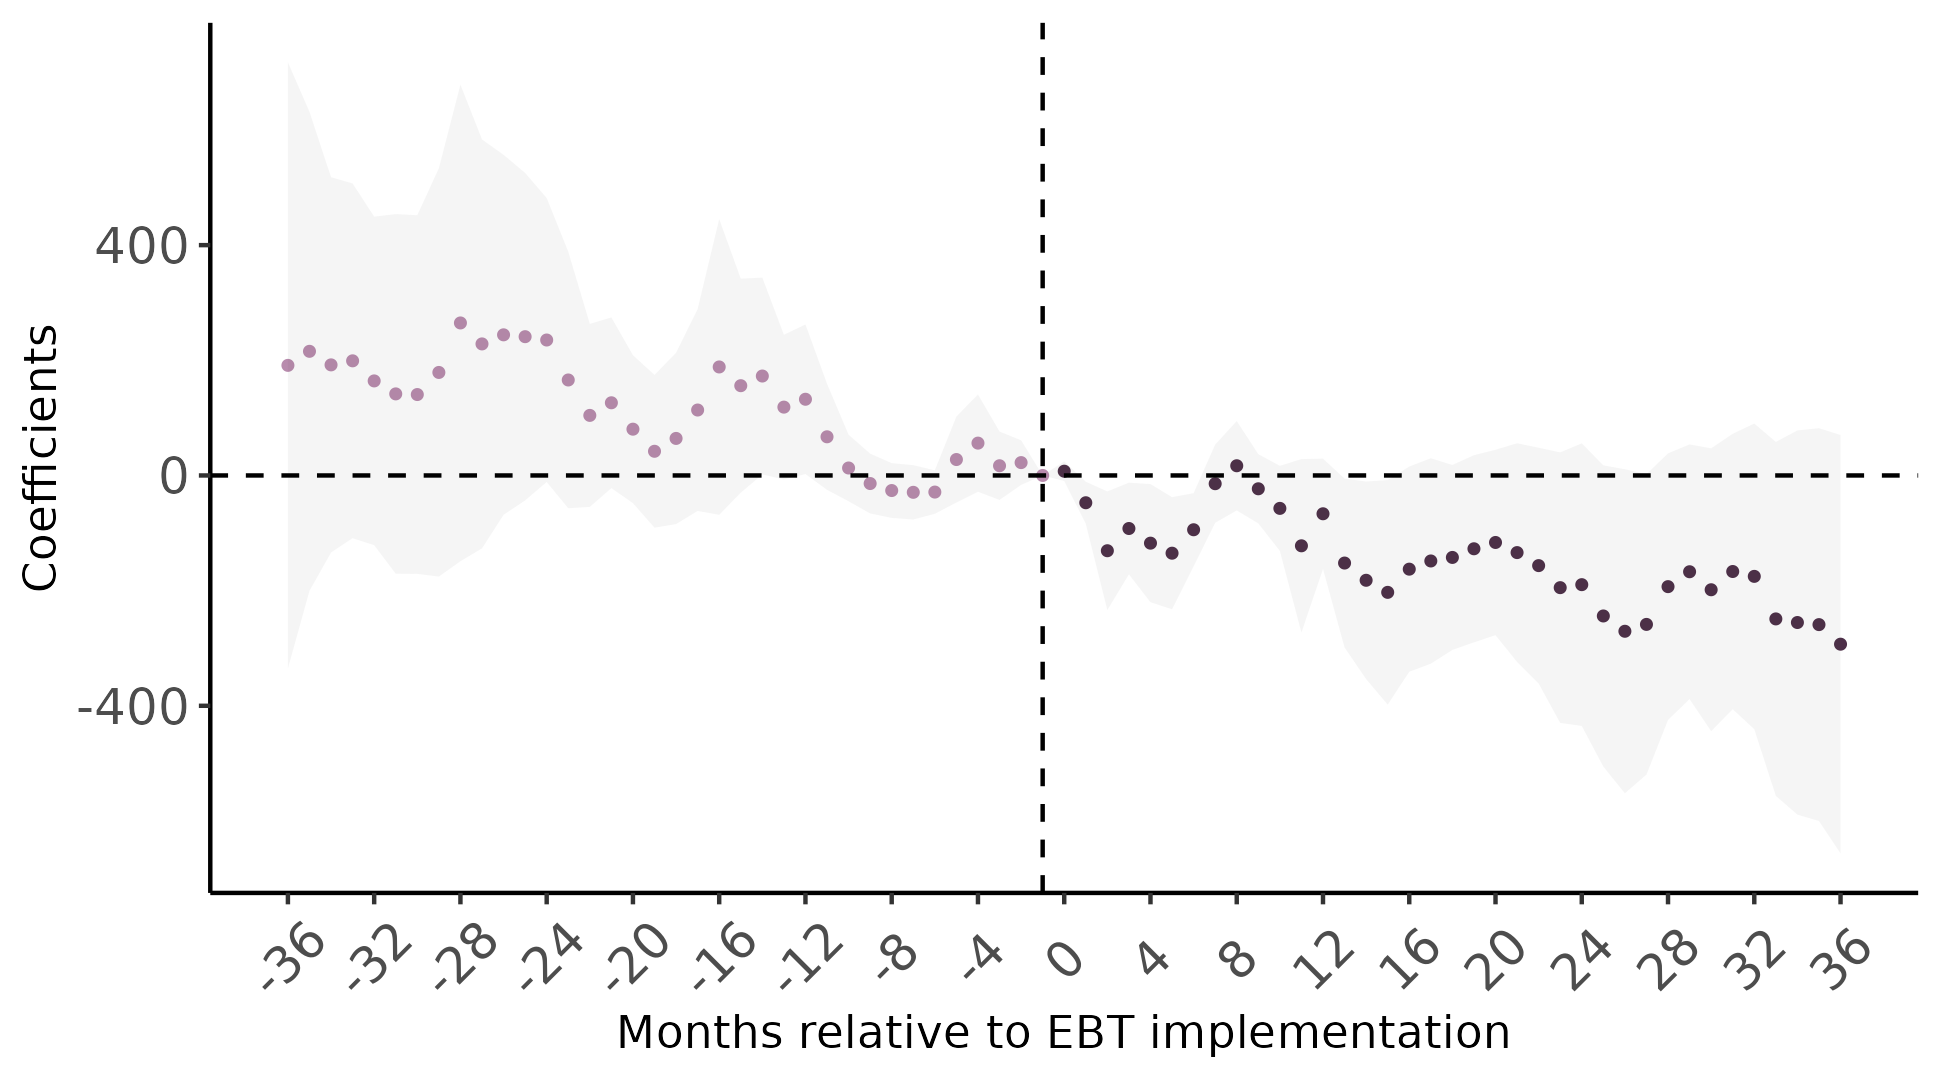
\includegraphics[width=\textwidth]{frac_mom_wic.png}  
		\caption{EBT and WIC Births Ratio}
		\label{mk_es1}
	\end{subfigure}
	\begin{subfigure}[t]{.5\textwidth}
		\centering
		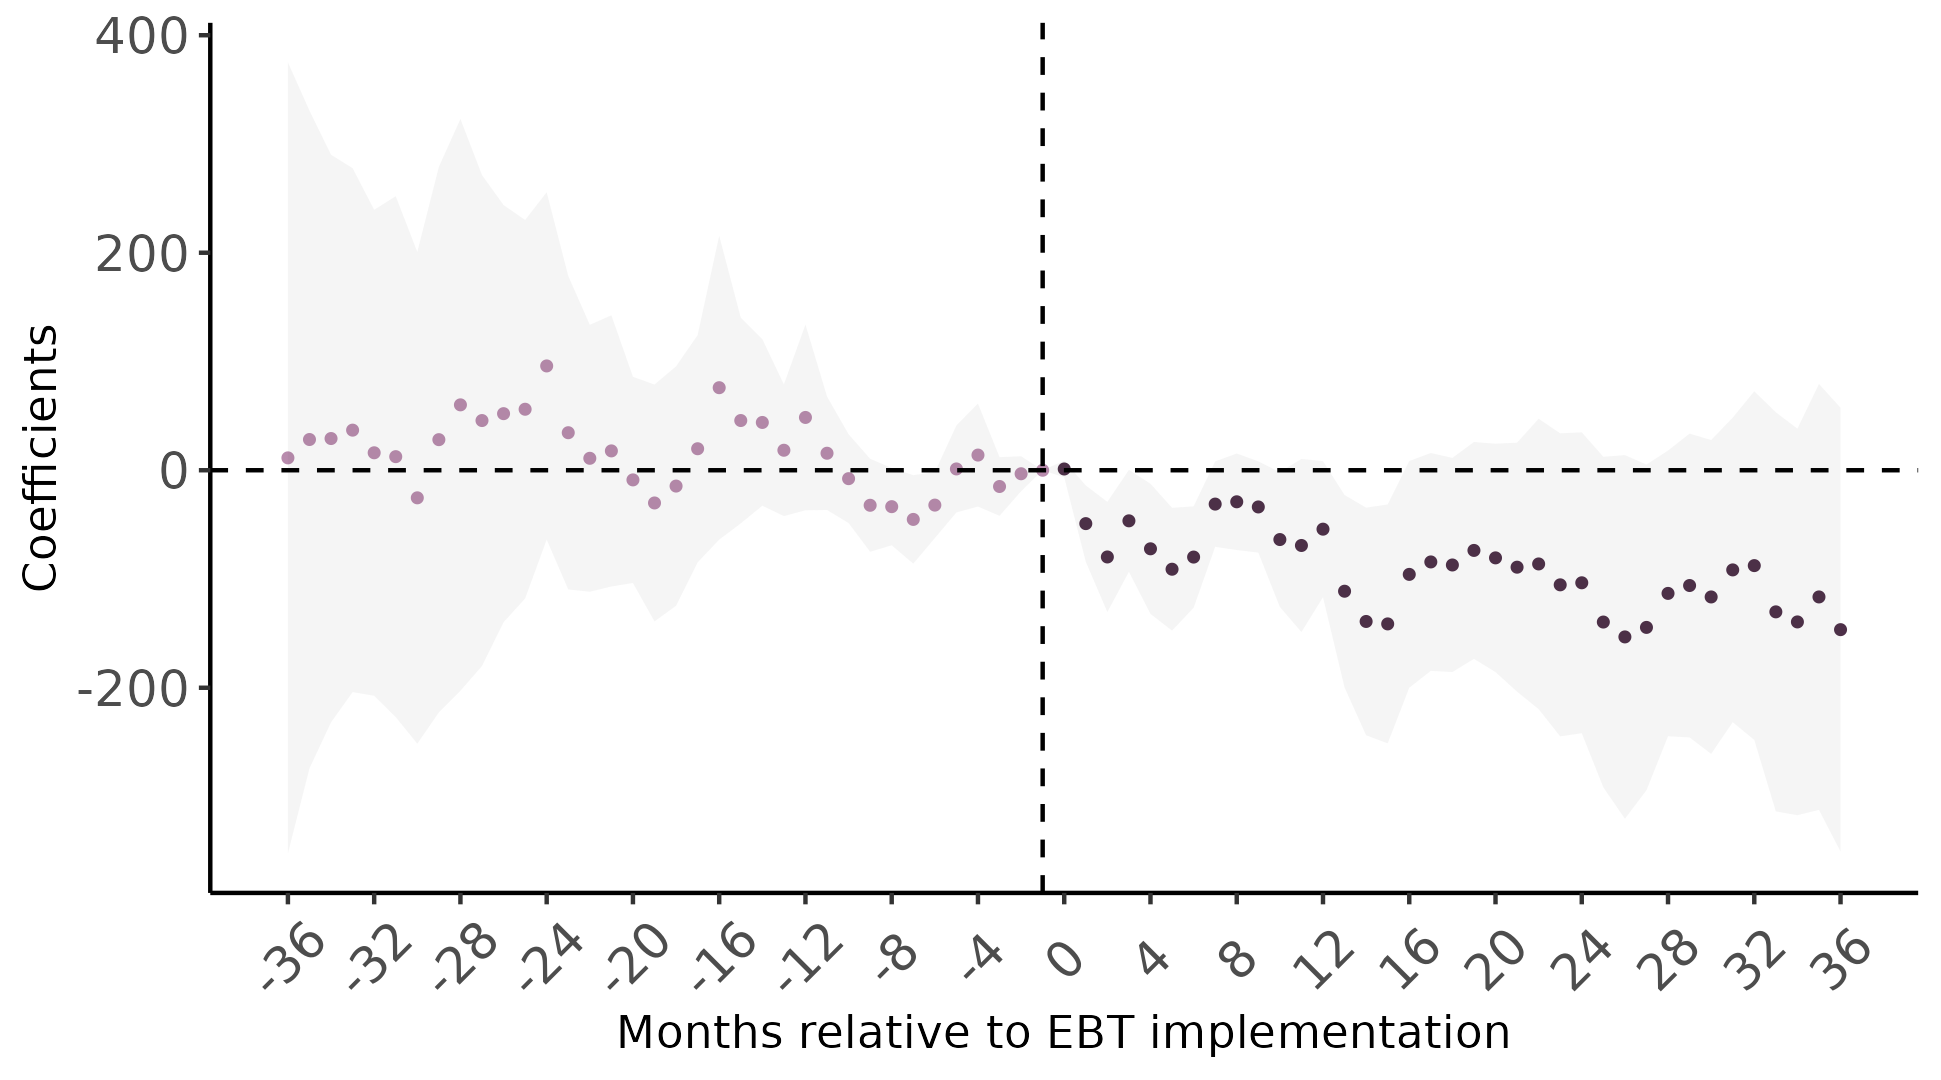
\includegraphics[width=\textwidth]{frac_poor_wic.png}  
		\caption{EBT and High Poverty WIC Birth Ratio}
		\label{mk_es2}
	\end{subfigure}
	\caption{\textsc{Event Study Plot for WIC Birth Ratio}}
	\label{mk_es}
	\footnotesize
	\vspace{6pt}
	\vspace{4pt}
	Notes: 
\end{figure}


\begin{table}[!htbp]
	\begin{center}
		\caption{\textsc{CS Estimators using Texas DSHS Data}} 
		\label{} 
		\scriptsize
		\begin{tabularx}{.9\linewidth}{@{}l*{6}{>{\centering\arraybackslash}X}@{}}
			\\[-1.8ex]\hline 
			\hline 
			\\[-1.8ex] 
			& \multicolumn{3}{c}{WIC Birth Ratio} & \multicolumn{3}{c}{High Poverty} \\
			& \multicolumn{3}{c}{} & \multicolumn{3}{c}{WIC Birth Ratio} \\
			\cmidrule(lr){2-4}\cmidrule(lr){5-7}
			& Full    & Full    & $\geq$ 15  &  Full    & Full    & $\geq$ 15  \\		
			& (1)     & (2)      & (3)    & (4)     & (5)    & (6)    \\
			\midrule
			
			Born after EBT  & -0.0102   &  -0.0297 & -0.0105  & -0.0067  &  -0.0446  &   0.0682$^{**}$   \\
			& (0.0069)  &  (0.0213) & (0.0319) & (0.0109) &  (0.0394)  &   (0.0283)   \\
			\\
			Covariates      &   &  \checkmark & \checkmark  &   &  \checkmark  &  \checkmark  \\
			Observations    & 10,050  & 10,050  & 5,200  &  5,750  &  5,750  &   4,350    \\
			Dep. Var. Mean (DVM)  & 0.5558  & 0.5558 &  0.5404 &  0.7935  &  0.7935  &   0.7960    \\
			\%(ATT/DVM)  &  -1.84\% &  -5.34\% &  -1.94\% & -0.84\%  &  -5.62\%  &   8.57\%   \\
			\hline \\[-1.8ex] 
			\hline 
			\hline \\ [-5.0ex] 		
		\end{tabularx}
	\end{center}
	\footnotesize
	\vspace{4pt}
	Notes: We report results with cells with more than 15 instead of 25 births to avoid having singular matrices.
\end{table}


\begin{figure}[!htbp]
	\begin{subfigure}[t]{.5\textwidth}
		\centering
		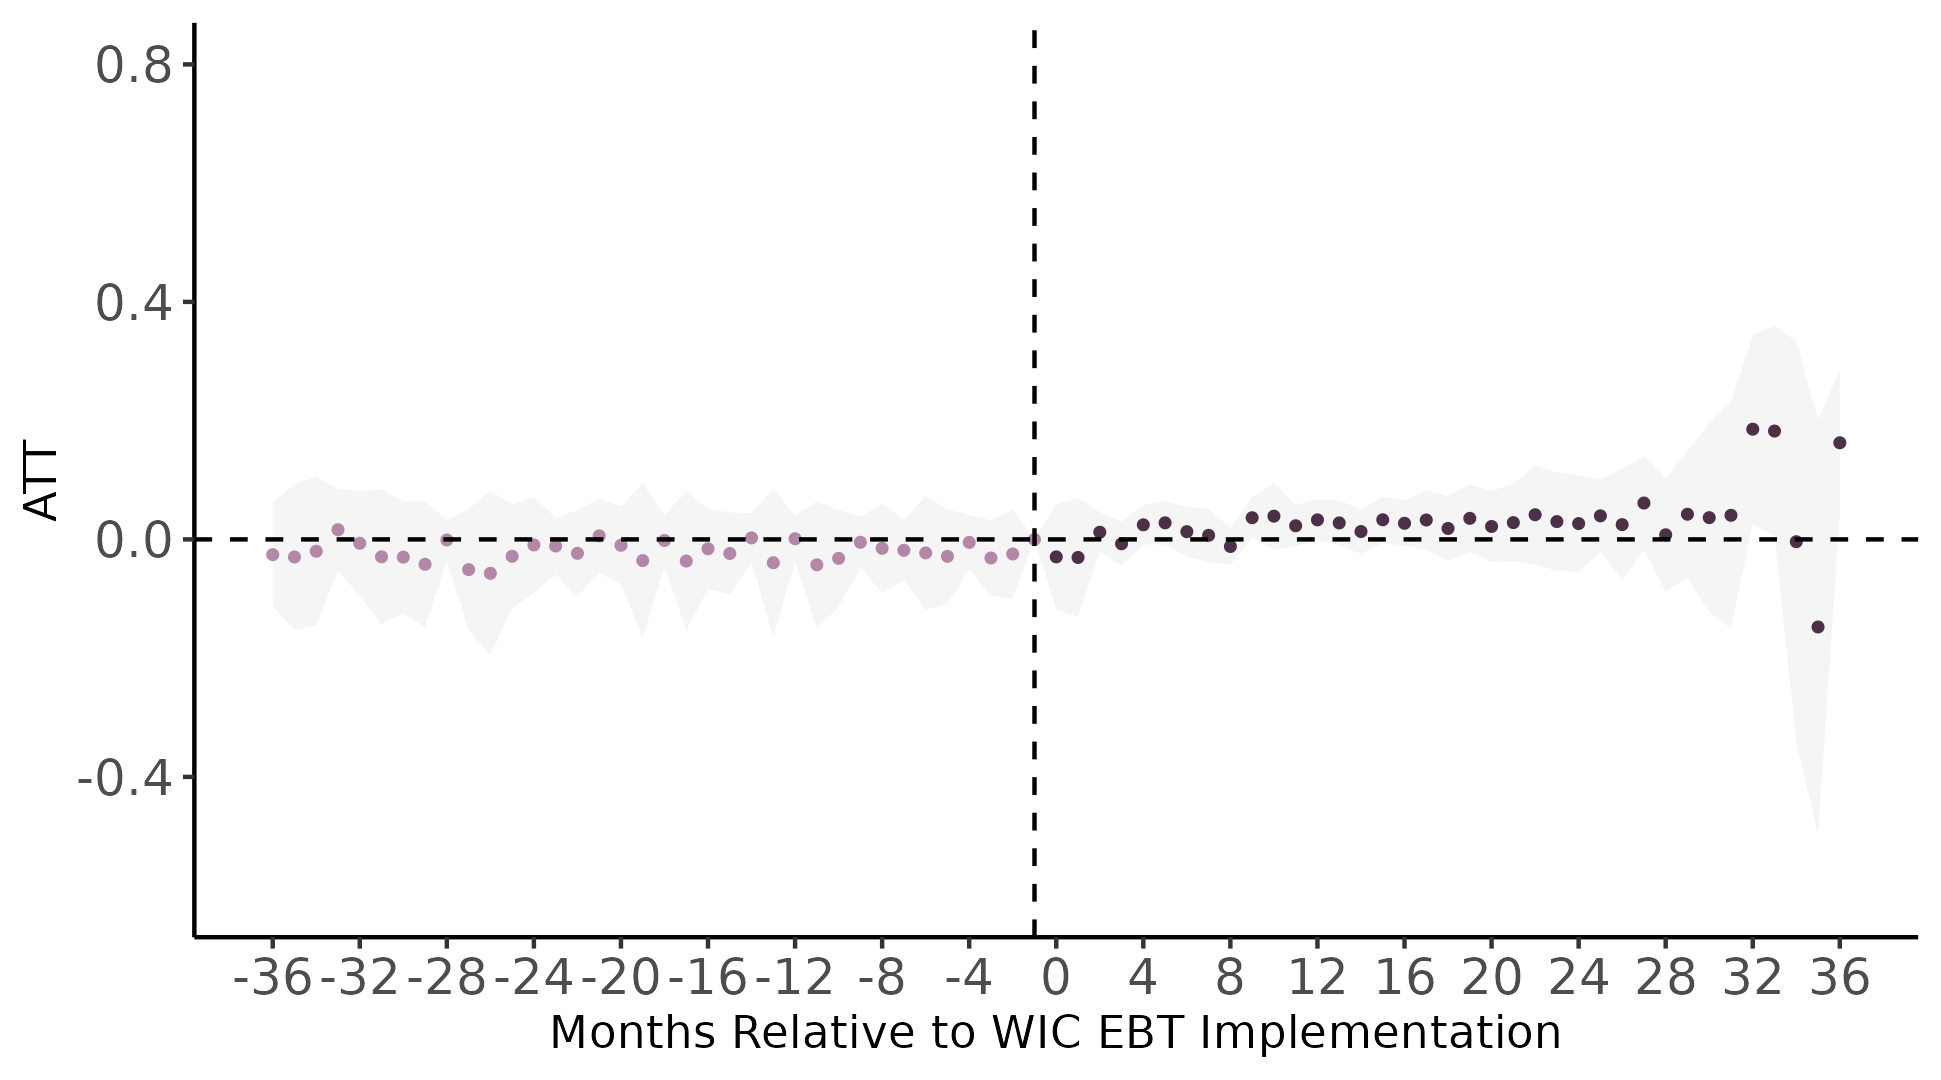
\includegraphics[width=\textwidth]{wic_tx_cs_es_frac_mom_wic.png}  
		\caption{WIC Births Ratio}
		\label{mk_es1}
	\end{subfigure}
	\begin{subfigure}[t]{.5\textwidth}
		\centering
		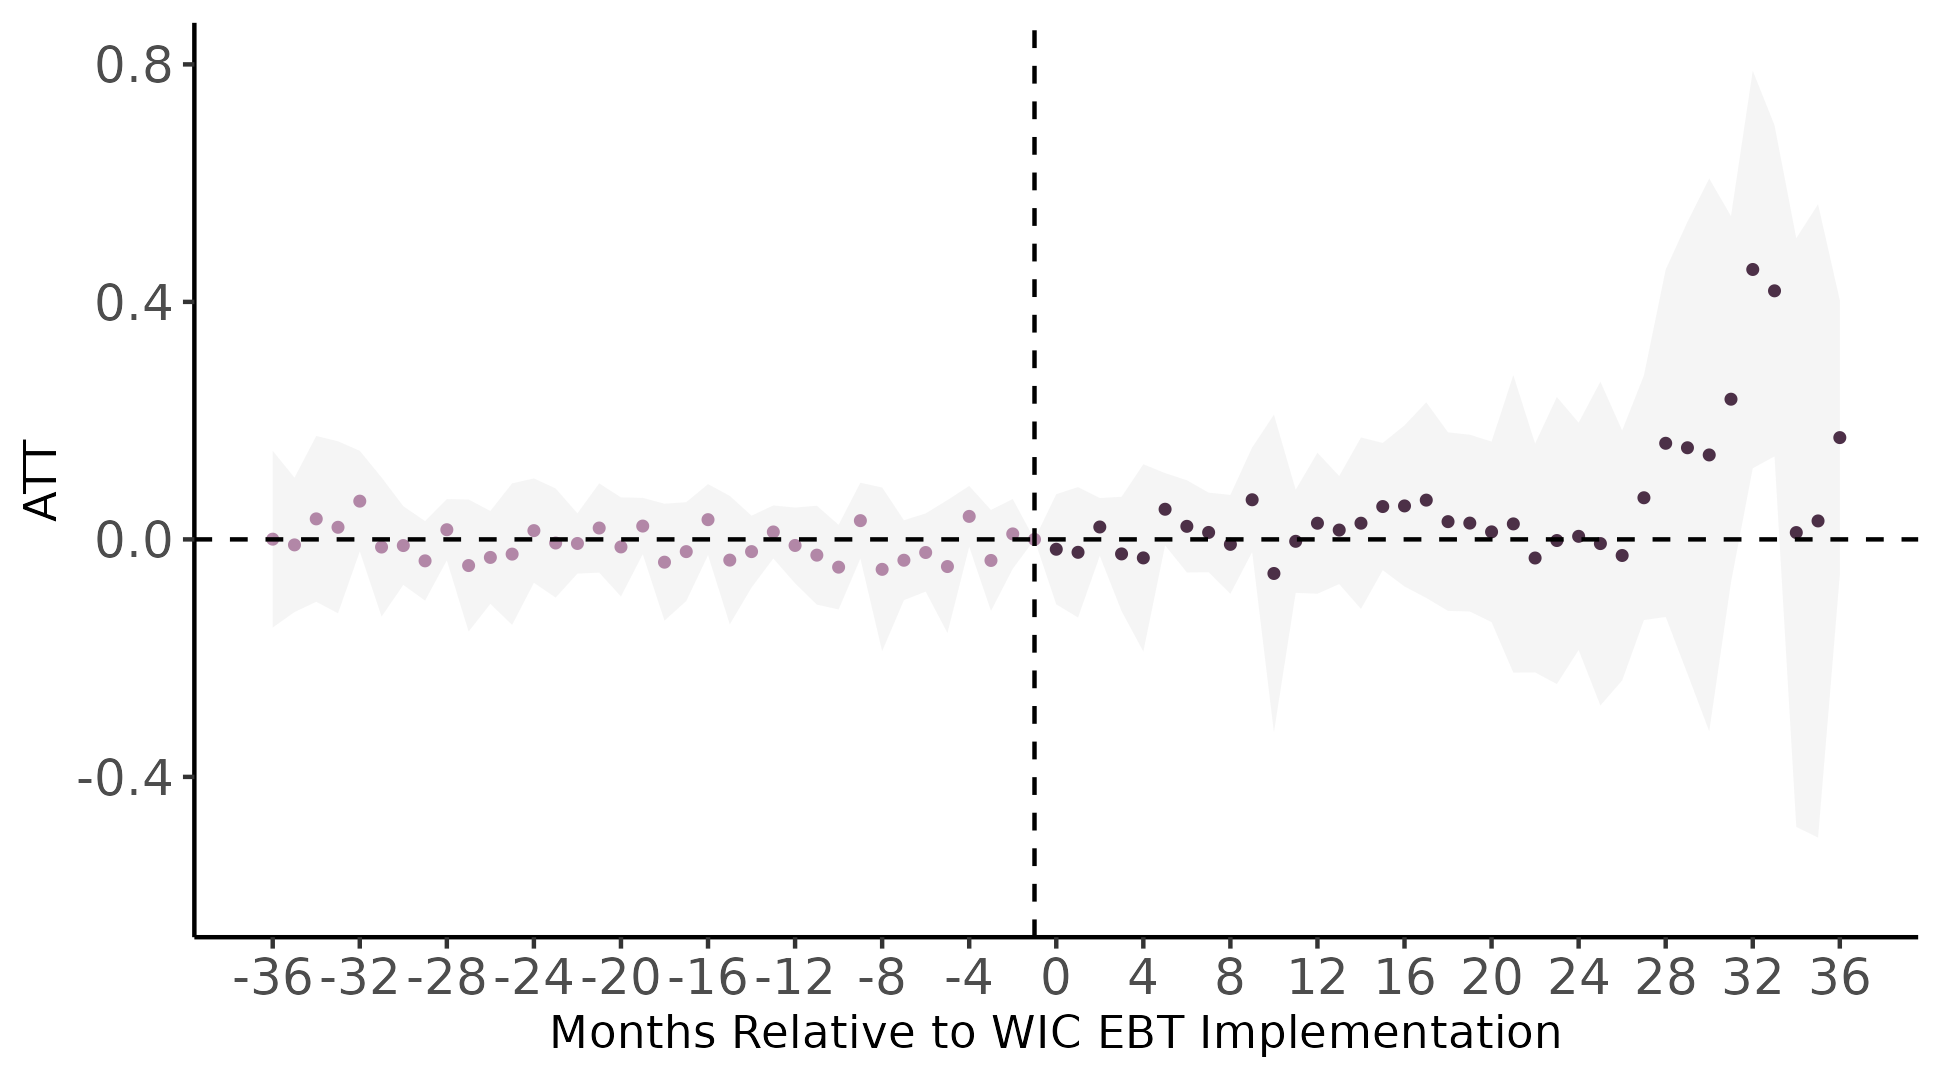
\includegraphics[width=\textwidth]{wic_tx_cs_es_frac_poor_wic.png}  
		\caption{High Poverty WIC Birth Ratio}
		\label{mk_es2}
	\end{subfigure}
	\caption{\textsc{Dynamic CS Estimates for WIC Birth Ratio}}
	\label{mk_es}
	\footnotesize
	\vspace{6pt}
	\vspace{4pt}
	Notes: As covariates we include all covariates from 2000 to 2004 as in our main results except income per person and net increase in WIC vendor due to unavailability of data. We replace income per person with median household income to account for baseline income difference.
\end{figure}


test sync collaborator

\clearpage

\begin{spacing}{1.25}
\newpage
\bibliographystyle{aea}
\bibliography{wic_br_ref}
\end{spacing}


\end{document}